\documentclass[11pt, letterpaper]{article}
\usepackage[utf8]{inputenc}
\usepackage{geometry}
\usepackage{fancyhdr}
\usepackage{amsmath, amssymb}
\usepackage{xcolor}
\usepackage{listings}
\usepackage{enumitem}
\usepackage{hyperref}
\usepackage{graphicx}
\usepackage{booktabs}

\setlength{\parindent}{0pt}
\setlist{itemsep=0.5em}
\setlength{\parskip}{0.5em}

\geometry{margin=1in}
\pagestyle{fancy}
\fancyhf{}
\lhead{\textbf{Solutions}}
\rhead{\textbf{Data Analysis and Regression, Homework 4}}
\cfoot{\thepage}

\definecolor{codegreen}{rgb}{0,0.6,0}
\definecolor{codegray}{rgb}{0.5,0.5,0.5}
\definecolor{codepurple}{rgb}{0.58,0,0.82}
\definecolor{backcolour}{rgb}{0.95,0.95,0.92}

\lstdefinestyle{mystyle}{
    backgroundcolor=\color{backcolour},
    commentstyle=\color{codegreen},
    keywordstyle=\color{magenta},
    numberstyle=\tiny\color{codegray},
    stringstyle=\color{codepurple},
    basicstyle=\ttfamily\footnotesize,
    breakatwhitespace=false,
    breaklines=true,
    captionpos=b,
    keepspaces=true,
    numbers=left,
    numbersep=5pt,
    showspaces=false,
    showstringspaces=false,
    showtabs=false,
    tabsize=2
}
\lstset{style=mystyle}

\newcommand{\problem}[1]{\section*{Problem #1}}
\newcommand{\subproblem}[1]{\subsection*{Problem #1}}
\newcommand{\answer}{\textbf{\textit{\textcolor{red}{Answer:}}}}
\begin{document}

\section*{Instructions}
\begin{itemize}
    \item Homework 4 was due Monday, August 17th at 18:00 Chicago Time.
    \item All numbers and figures come from \texttt{homework\_4\_solution.ipynb}, run from top to bottom.
\end{itemize}
\hrule
\vspace{0.5cm}

\pagebreak

\problem{1: New Data in Our Curve}

We'll start by fitting a curve made up of pieces (piecewise linear). Where these pieces intersect are our knots. With $K$ knots the model is:
$$
f(x) = w_0 + w_1 x + \sum_{j=1}^{K} w_{1+j} (x - \kappa_j)_{+},
\qquad (u)_{+} = \max(u, 0)
$$

Each column $(x - \kappa_j)_+$ is zero before the knot $\kappa_j$. After the knot it has a slope of 1, so that $w_{1+j}$ is the change in slope at that knot. The model has $p = 2 + K$ parameters.

    \begin{lstlisting}[language=Python]
import numpy as np

def basis(x, knots):
    """Build the basis matrix. One extra column per knot."""
    cols = [np.ones_like(x), x] + [np.clip(x - k, 0.0, None) for k in knots]
    return np.column_stack(cols)

def knots(K):
    """K knots, evenly spaced inside (0, 1)."""
    return np.linspace(0, 1, K + 2)[1:-1]

def fit_ols(A, y):
    beta, *_ = np.linalg.lstsq(A, y, rcond=None)
    return beta\end{lstlisting}
The $x$ values are the same for all draws; note that only the noise is random (same as Homework 2).

    \begin{lstlisting}[language=Python]
N_TRAIN, N_TEST = 60, 500
SIGMA   = 0.3
K_MAX   = 18
N_REPS  = 600

x_train = np.linspace(0, 1, N_TRAIN)
x_test  = np.linspace(0.005, 0.995, N_TEST)

def f_true(x):
    return np.sin(2 * np.pi * x)

# in repetition s, use rng = np.random.RandomState(s) and draw
#   y_train = f_true(x_train) + rng.normal(0, SIGMA, N_TRAIN)
#   y_test  = f_true(x_test)  + rng.normal(0, SIGMA, N_TEST)\end{lstlisting}

\subproblem{1.1: Basis Functions}
\begin{itemize}
    \item Plot the columns of \texttt{basis(x\_train, knots(4))} against $x$.
    \item In one sentence, what does the coefficient on the column $(x - \kappa_j)_+$ tell you?
\end{itemize}

\answer

\begin{center}
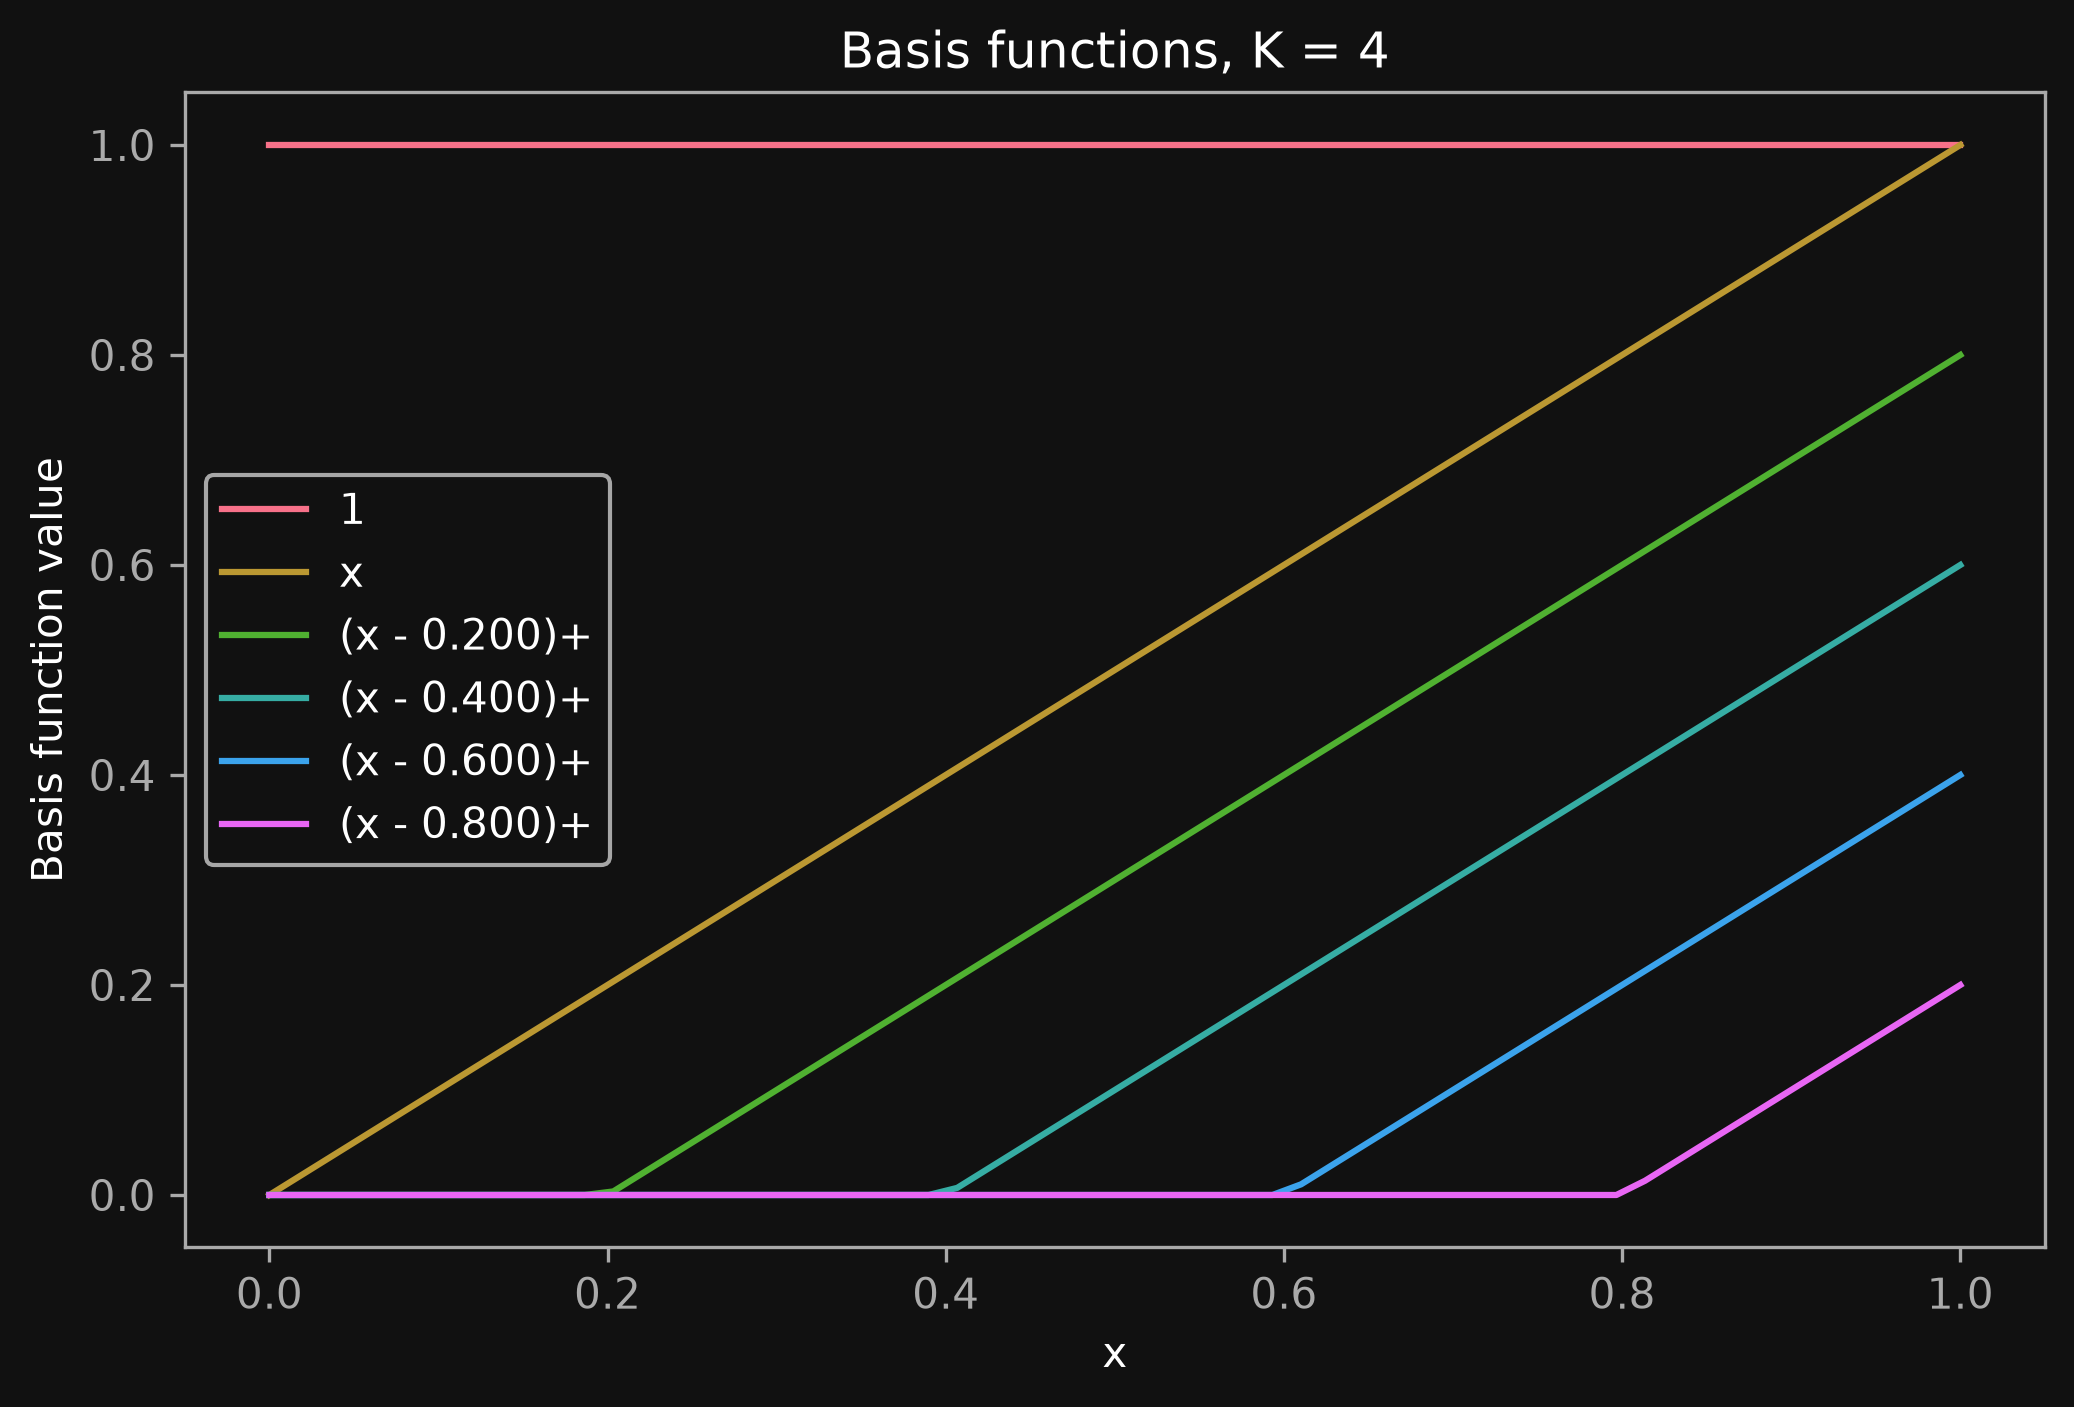
\includegraphics[width=0.68\textwidth]{./figures/problem1_basis.png}
\end{center}

The coefficient on $(x - \kappa_j)_+$ is the change in slope at the knot $\kappa_j$.


\subproblem{1.2: One Set of Data}
Use \texttt{np.random.RandomState(0)} for the noise. Fit the model for $K = 1$, $K = 4$ and $K = 18$.
\begin{itemize}
    \item Plot the training data and the three curves on one plot.
    \item Just from eyeballing; which do you think is the best from balancing bias and variance?
\end{itemize}

\answer

\begin{center}
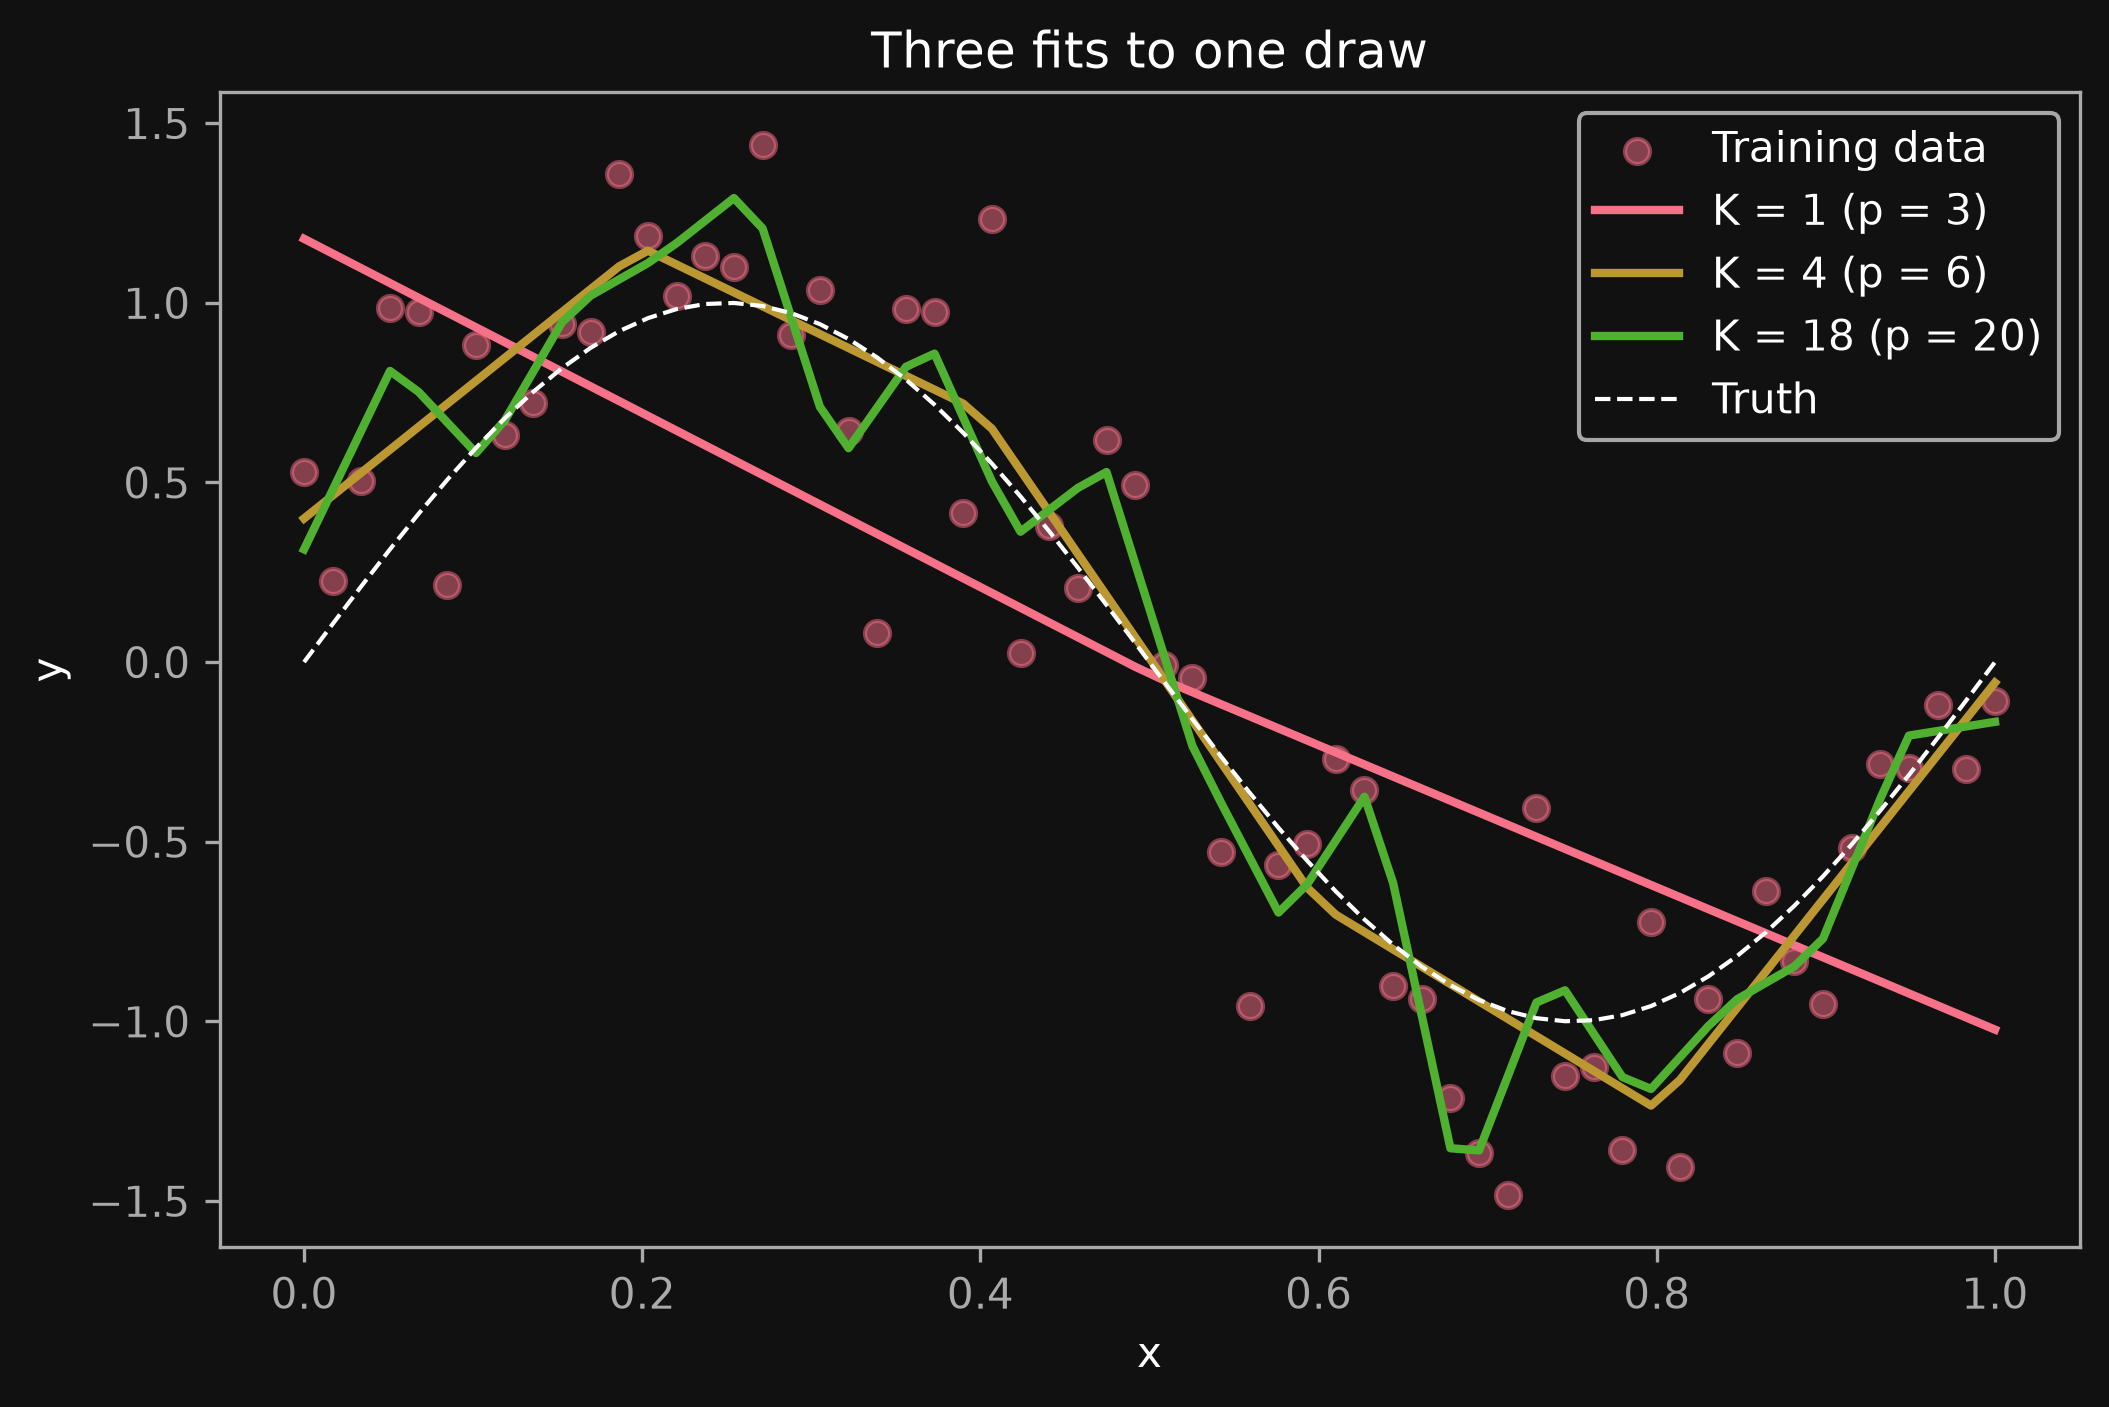
\includegraphics[width=0.68\textwidth]{./figures/problem1_three_fits.png}
\end{center}

$K = 4$. $K = 1$ can bend only once, so it is almost a straight line and misses the shape; $K = 18$
has a knot every three data points and follows single points.


\subproblem{1.3: Sim}
For each $K = 0, 1, \dots, 30$ and each repetition $s = 0, \dots, 999$:
\begin{enumerate}
    \item Draw new \texttt{y\_train} and \texttt{y\_test} with \texttt{np.random.RandomState(s)}.
    \item Fit the model on the training data only.
    \item Record the MSE on the training data and the MSE on the test data.
\end{enumerate}
Take the mean of each over the 600 repetitions.
\begin{itemize}
    \item Plot the two mean curves against $K$ on one plot (ie. mean MSE and test MSE for each $K$).
    \item Give a table of the two values for $K \in \{0, 2, 3, 5, 10, 15, 30\}$.
\end{itemize}

\answer

The code block above sets \texttt{K\_MAX = 18} and \texttt{N\_REPS = 600}, so the table below runs
to $K = 18$ in place of $K = 30$, over 600 repetitions. $K = 4$ is included because it is the
minimum.

\begin{lstlisting}[language=Python]
A_train = {K: basis(x_train, knots(K)) for K in range(K_MAX + 1)}
A_test = {K: basis(x_test, knots(K)) for K in range(K_MAX + 1)}

ins_all, oos_all = [], []
for s in range(N_REPS):
    rng = np.random.RandomState(s)
    y_tr = f_true(x_train) + rng.normal(0, SIGMA, N_TRAIN)
    y_te = f_true(x_test) + rng.normal(0, SIGMA, N_TEST)
    ins_row, oos_row = [], []
    for K in range(K_MAX + 1):
        beta = fit_ols(A_train[K], y_tr)
        ins_row.append(np.mean((A_train[K] @ beta - y_tr) ** 2))
        oos_row.append(np.mean((A_test[K] @ beta - y_te) ** 2))
    ins_all.append(ins_row)
    oos_all.append(oos_row)

in_sample = np.mean(ins_all, axis=0)
out_sample = np.mean(oos_all, axis=0)
\end{lstlisting}

\begin{center}
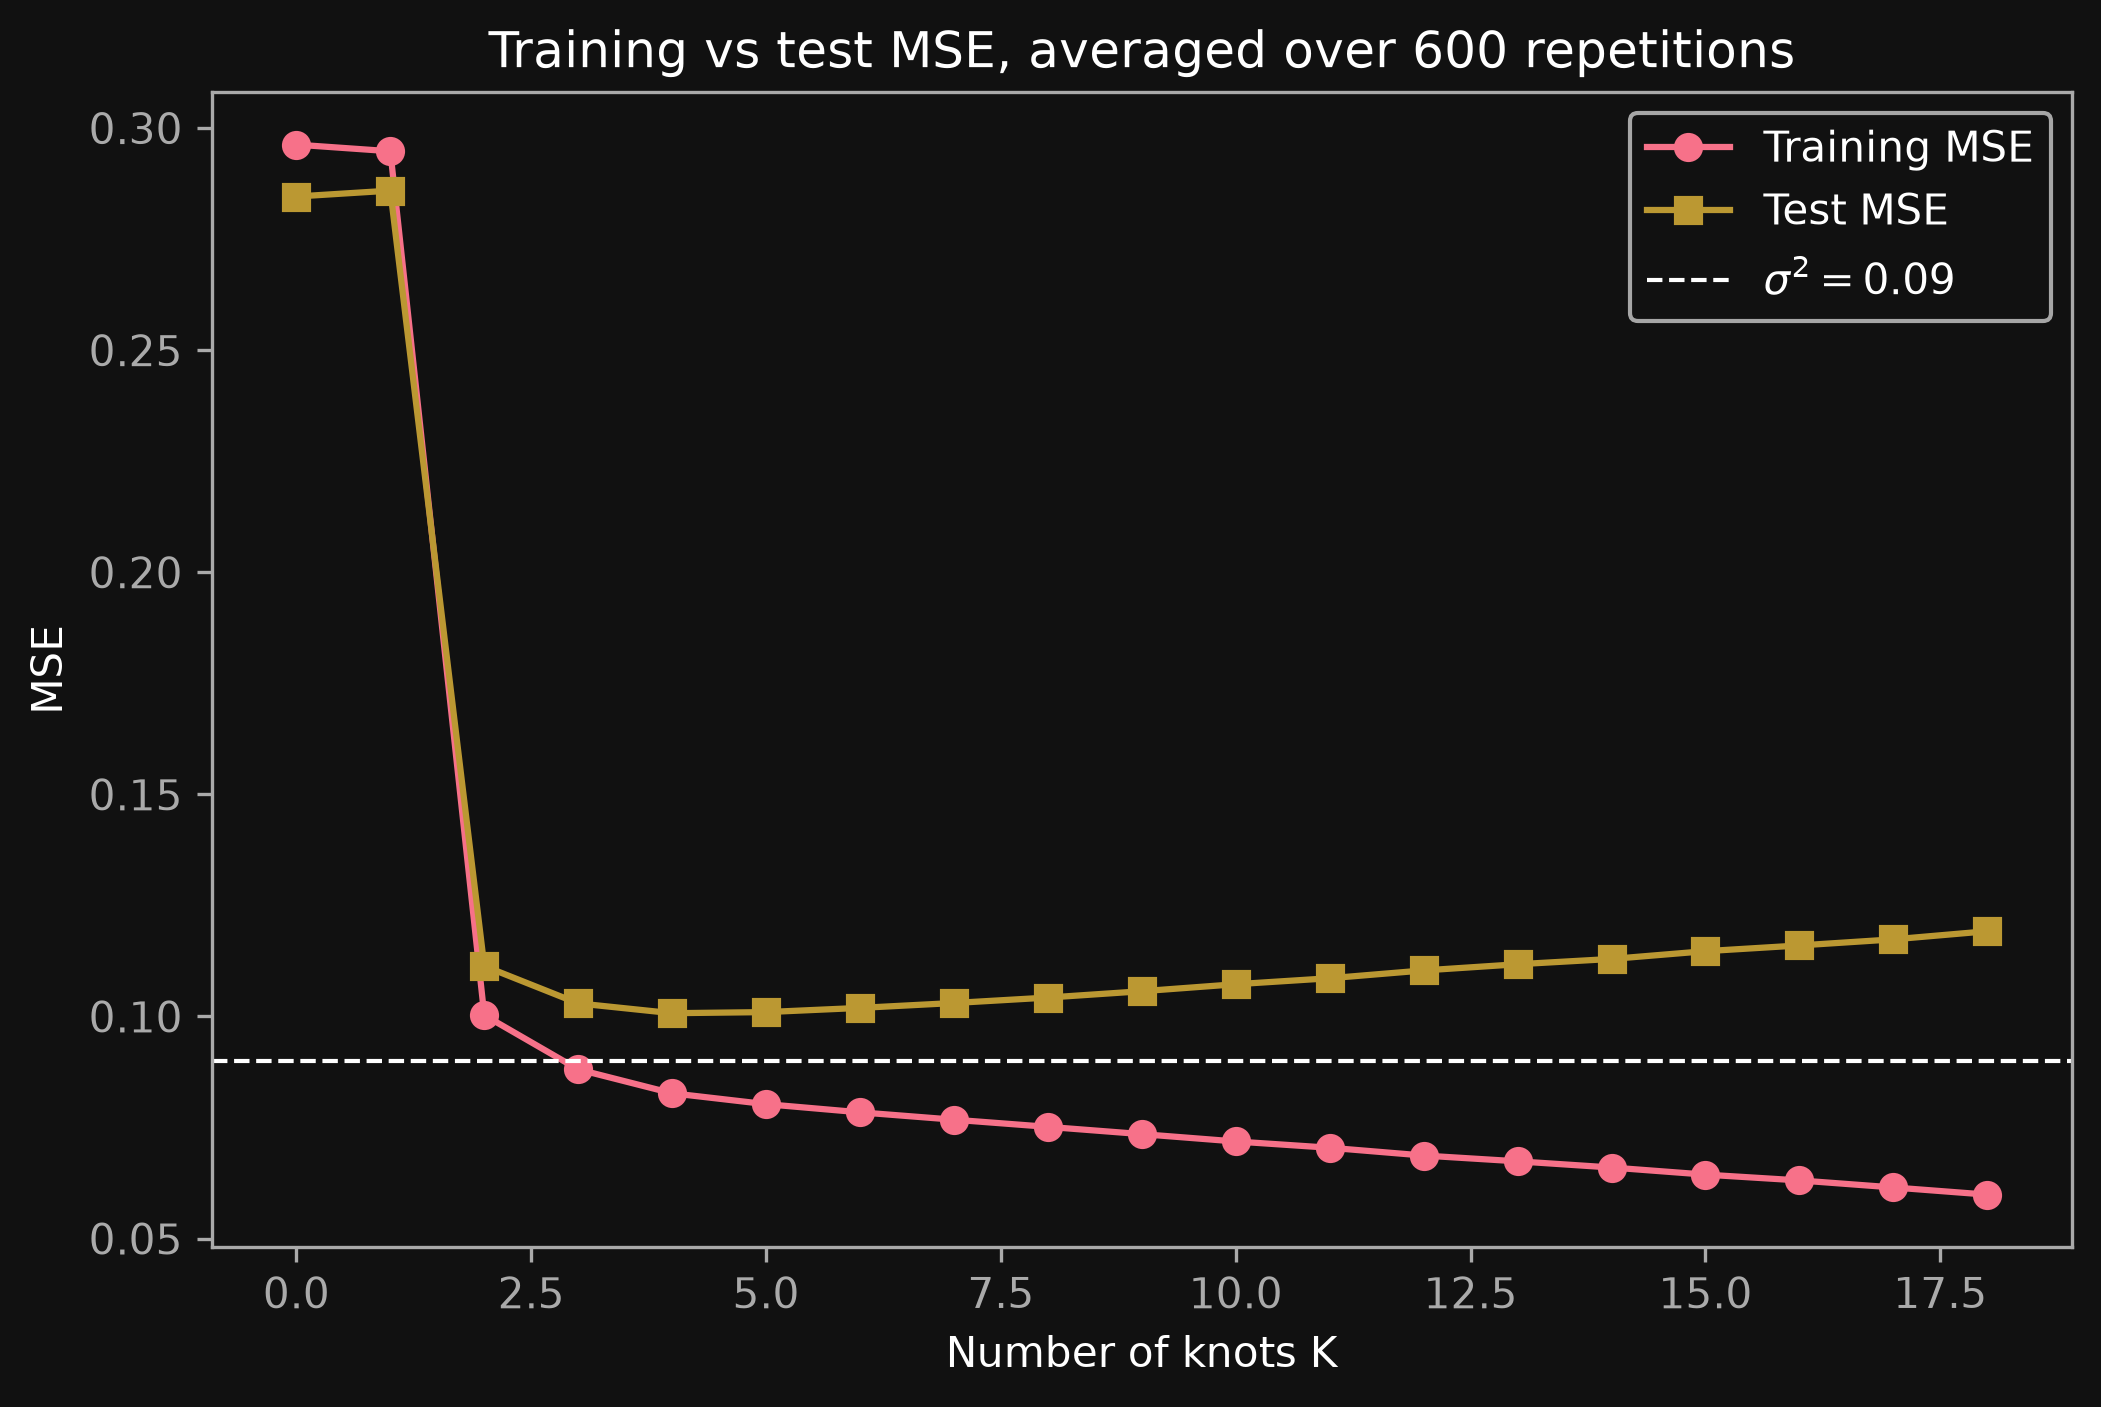
\includegraphics[width=0.68\textwidth]{./figures/problem1_mse_curves.png}
\end{center}

\begin{center}
\begin{tabular}{rrrr}
\toprule
$K$ & $p$ & training MSE & test MSE \\
\midrule
0  & 2  & 0.2963 & 0.2846 \\
2  & 4  & 0.1003 & 0.1113 \\
3  & 5  & 0.0881 & 0.1029 \\
4  & 6  & 0.0827 & \textbf{0.1007} \\
5  & 7  & 0.0802 & 0.1010 \\
10 & 12 & 0.0718 & 0.1073 \\
15 & 17 & 0.0644 & 0.1147 \\
18 & 20 & 0.0599 & 0.1192 \\
\bottomrule
\end{tabular}
\end{center}


\subproblem{1.4: What the Plot Shows}
\begin{itemize}
    \item Does the training MSE ever increase when you add a knot? 
    \item In one sentence, why is that?
    \item Give the value of $K$ with the lowest test MSE.
\end{itemize}

\answer

\begin{itemize}
    \item No. The training MSE falls at every step, from $0.2963$ to $0.0599$.
    \item Each extra knot adds a parameter, and more parameters let the fit pass closer to the
          training points. Adding a column can never raise the minimized sum of squares, because the
          old solution is still available with a zero coefficient on the new column.
    \item The test MSE is lowest at $\mathbf{K = 4}$ ($p = 6$), at $0.1007$. It then rises at every
          step, to $0.1192$ at $K = 18$.
\end{itemize}


\subproblem{1.5: Theory}
For a model with $p$ parameters that has the correct shape, the expected test MSE is roughly:
$$
\sigma^2 \left( 1 + \frac{p}{n} \right)
$$
Here $p = 2 + K$ and $n = 60$.
\begin{itemize}
    \item Draw this theoretical curve on top of your test MSE curve (from the previous question).
    \item Give the range of $K$ where $\left| \text{simulated} / \text{formula} - 1 \right| \le 0.03$.
    \item In 1--2 sentences, what does the formula leave out at small $K$?
\end{itemize}

\answer

\begin{center}
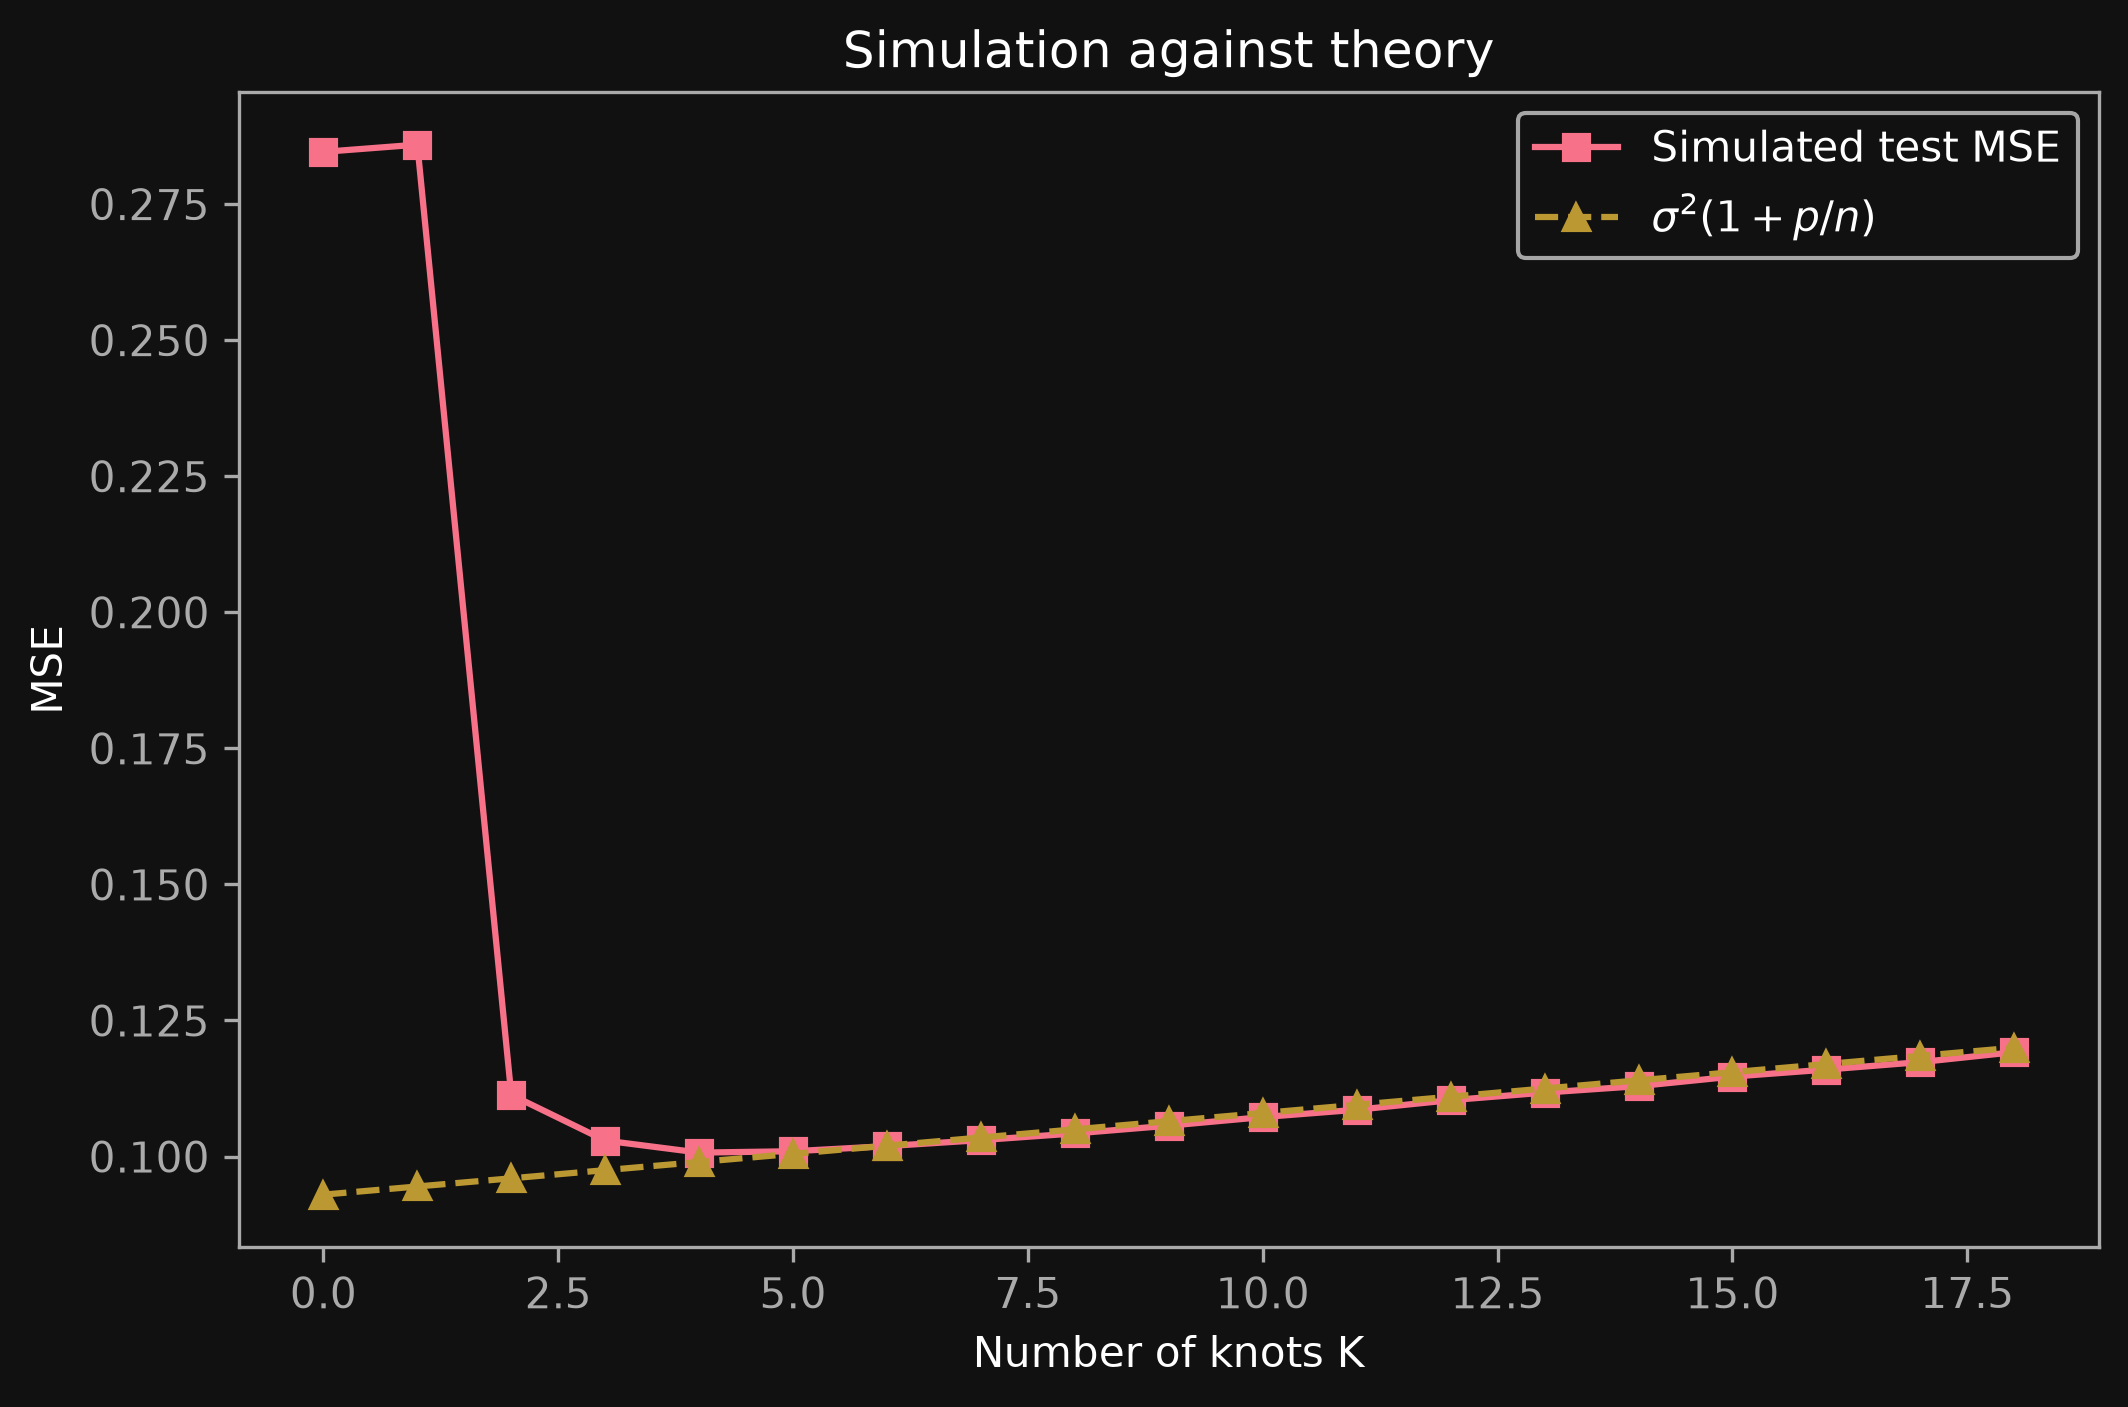
\includegraphics[width=0.68\textwidth]{./figures/problem1_theory.png}
\end{center}

\begin{center}
\begin{tabular}{rrrr}
\toprule
$K$ & simulated & $\sigma^2(1 + p/n)$ & gap \\
\midrule
0  & 0.2846 & 0.0930 & $+206.0\%$ \\
2  & 0.1113 & 0.0960 & $+16.0\%$ \\
3  & 0.1029 & 0.0975 & $+5.6\%$ \\
4  & 0.1007 & 0.0990 & $+1.7\%$ \\
5  & 0.1010 & 0.1005 & $+0.5\%$ \\
10 & 0.1073 & 0.1080 & $-0.7\%$ \\
15 & 0.1147 & 0.1155 & $-0.7\%$ \\
18 & 0.1192 & 0.1200 & $-0.7\%$ \\
\bottomrule
\end{tabular}
\end{center}

The simulation is within $3\%$ of the formula for $\mathbf{K = 4}$ to $\mathbf{K = 18}$, the whole
range available. ($K = 3$ is $5.6\%$ away, outside; $K = 4$ is $1.7\%$ away, inside.)

The formula charges only for estimating $p$ parameters, and it assumes the model can reproduce the
true shape. At small $K$ it cannot: a line with one or two bends is nowhere near $\sin(2\pi x)$, so
the gap at $K = 0$ and $K = 2$ is squared bias, which the formula leaves out entirely.


\pagebreak

\problem{2: Which Knots Are Real?}

In the previous question, the data was a sin wave. This time, the data really is piecewise linear; the slope changes at $x = 0.3$ and at
$x = 0.7$. There are 19 possible knots, and we need to see if we can find the real ones.

    \begin{lstlisting}[language=Python]
TRUE_KNOTS = [0.3, 0.7]
TRUE_BETA  = np.array([0.0, 2.0, -8.0, 10.0])   # intercept, slope, then the two slope changes
CANDIDATE_KNOTS = np.linspace(0.05, 0.95, 19)
N2, SIGMA2 = 200, 0.3

rng = np.random.RandomState(7)
x2 = rng.uniform(0, 1, N2)
y2 = basis(x2, TRUE_KNOTS) @ TRUE_BETA + rng.normal(0, SIGMA2, N2)

# scikit-learn adds its own intercept, so remove the first column
A_full = basis(x2, CANDIDATE_KNOTS)
design = A_full[:, 1:]\end{lstlisting}

\subproblem{2.1: Plain OLS}
Fit OLS with all 19 possible knots.
\begin{itemize}
    \item Give the largest coefficient of the 19 knot columns, in absolute value.
    \item Plot the fitted curve.
    \item Can you find the two real knots from the coefficients? Give a why or why not reason in one sentence.
\end{itemize}

\answer

The largest knot coefficient is $\mathbf{23.28}$ in absolute value. The largest true slope change is
$10$, so the ratio is $\mathbf{2.33}$.

\begin{center}
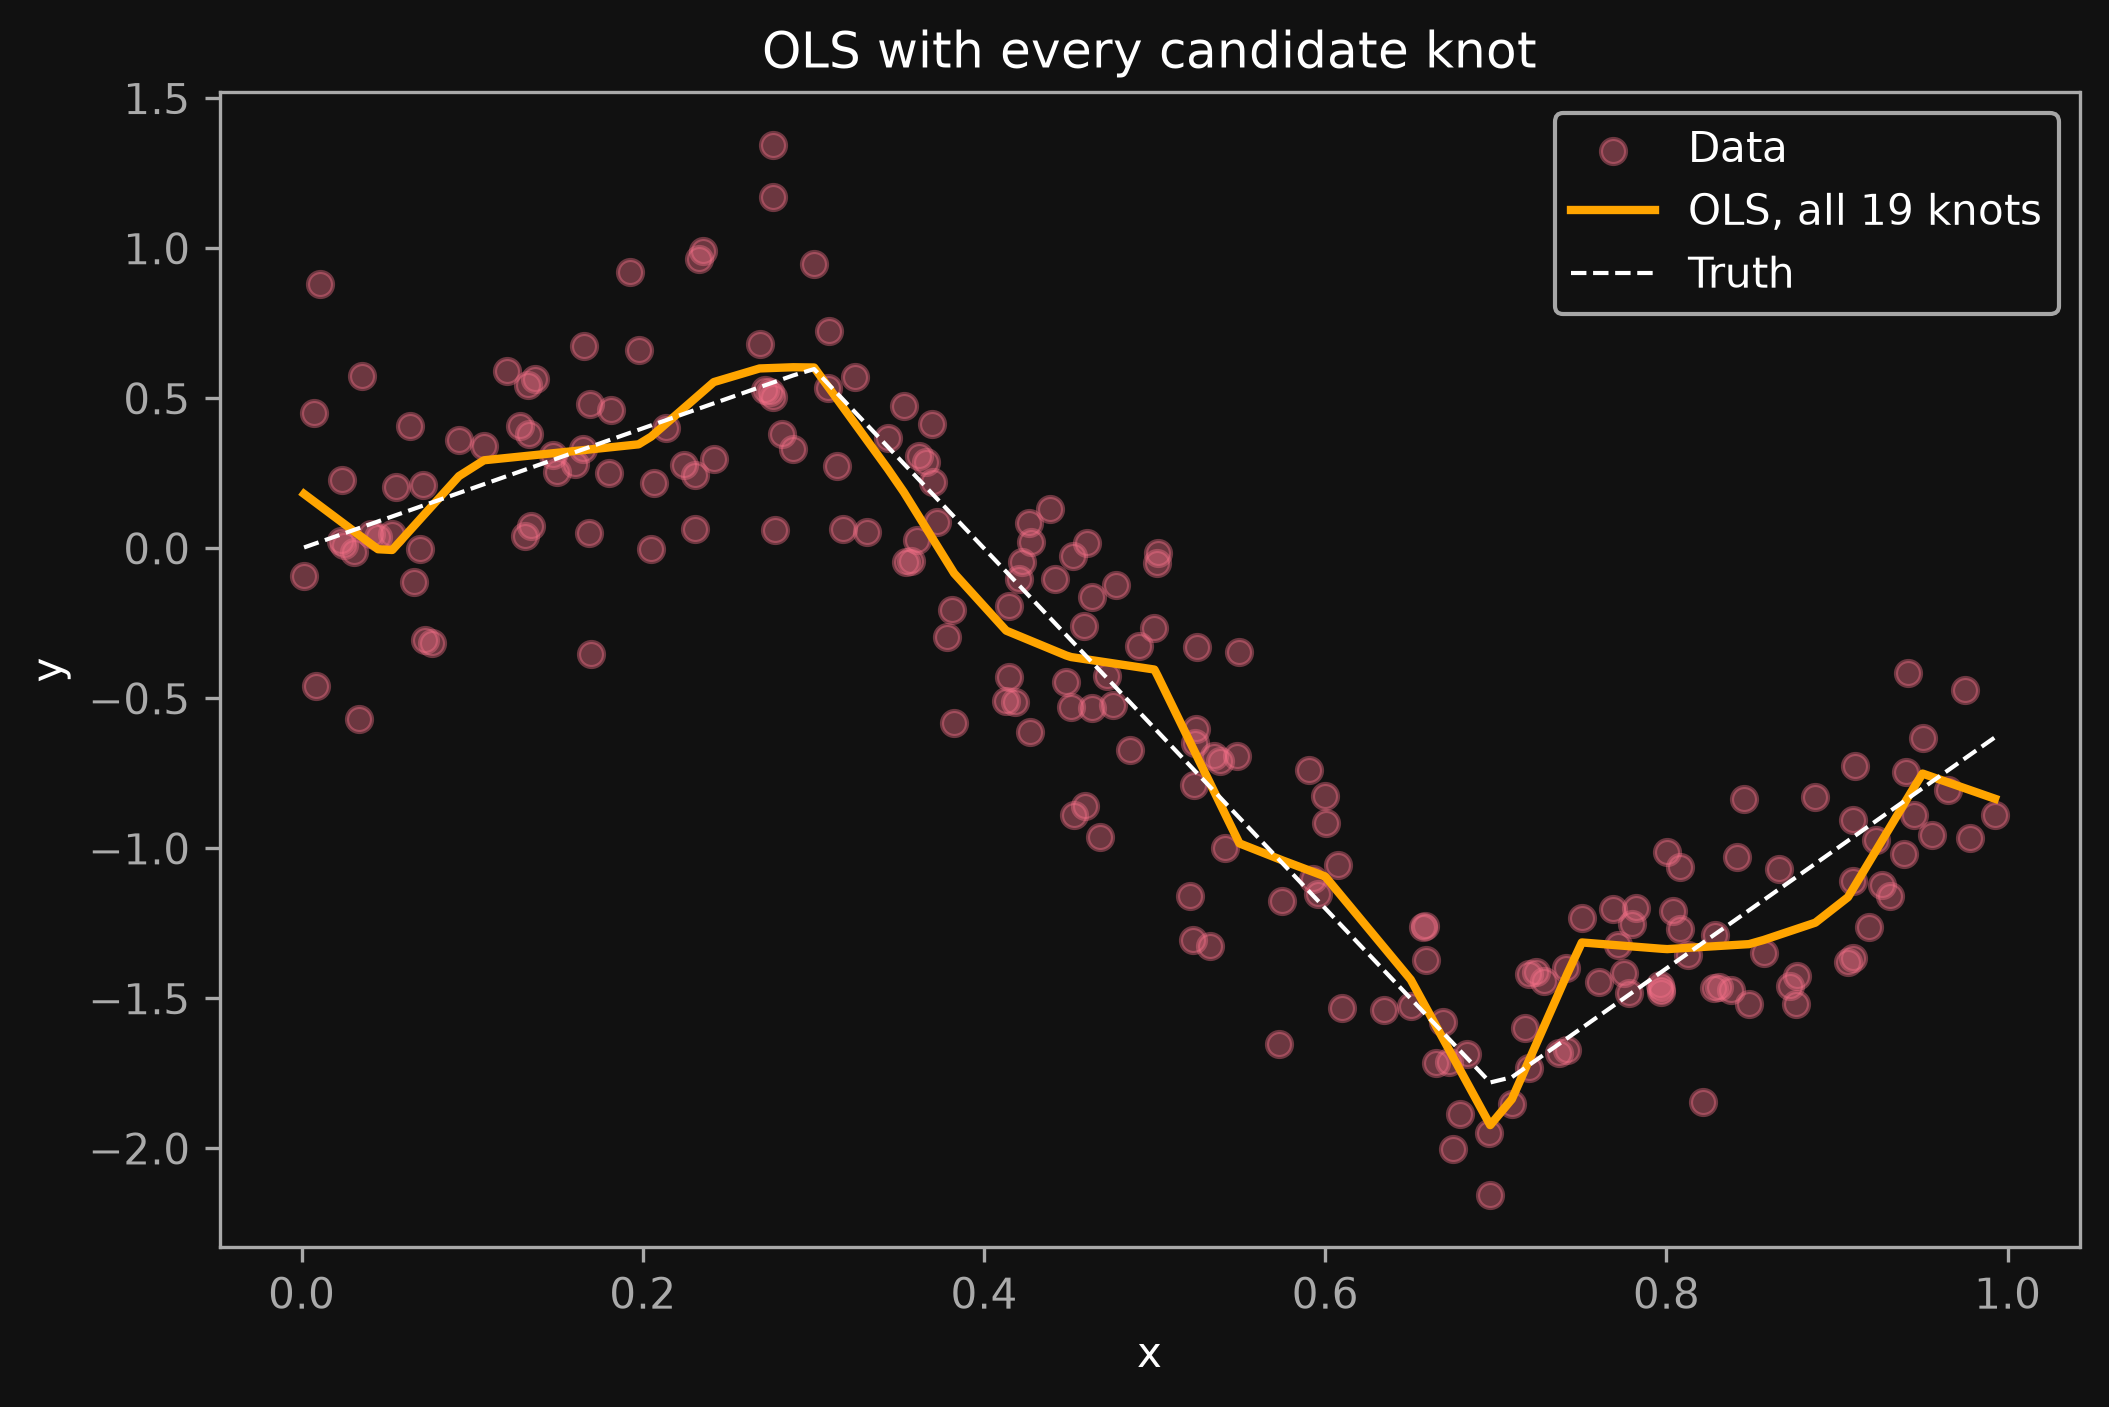
\includegraphics[width=0.68\textwidth]{./figures/problem2_ols_fit.png}
\end{center}

No. The coefficients alternate in sign again and again
($+10.55$, $-5.72$, $+0.02$, $+4.35$, $-4.74$, $-8.03$, \dots), so nothing marks out $0.30$
and $0.70$.
Knots that sit close together give almost the same column, and OLS is free to place a large positive
coefficient on one and cancel it with a large negative one on its neighbor without changing the
fitted values much.


\subproblem{2.2: Lasso to the Rescue?}
Fit \texttt{LassoCV(cv=5, random\_state=0, max\_iter=200000)} on \texttt{design}.
\begin{itemize}
    \item Give the $\alpha$/$\lambda$ that it selects.
    \item Give the number of knots with a coefficient that is not zero (or extremely close to it). Are both real knots in the list?
\end{itemize}

\answer

\begin{itemize}
    \item $\alpha = \mathbf{0.00054}$.
    \item \textbf{4 of 19} knots survive: $\{0.05,\ 0.25,\ 0.30,\ 0.70\}$.
    \item Yes, both real knots are in the list, along with two false ones. Note that $0.25$ sits next
          to the real knot at $0.30$; when two columns are nearly identical, Lasso often splits one
          real effect between them.
\end{itemize}


\subproblem{2.3: Change the Penalty}
Fit \texttt{Lasso(alpha=a, max\_iter=200000)} for
$a \in \{0.001,\, 0.005,\, 0.01,\, 0.02,\, 0.05,\, 0.1\}$.
\begin{itemize}
    \item Give a table with one row for each $\alpha$: the number of knots that stay, and their values.
    \item Is there an $\alpha$ that keeps exactly $\{0.3,\ 0.7\}$ and nothing else?
\end{itemize}

\answer

\begin{center}
\begin{tabular}{rrl}
\toprule
$\alpha$ & knots that stay & values \\
\midrule
0.001 & 2 & $\{0.30,\ 0.70\}$ \\
0.005 & 3 & $\{0.25,\ 0.30,\ 0.70\}$ \\
0.010 & 3 & $\{0.20,\ 0.25,\ 0.70\}$ \\
0.020 & 2 & $\{0.15,\ 0.20\}$ \\
0.050 & 2 & $\{0.10,\ 0.15\}$ \\
0.100 & 0 & $\{\}$ \\
\bottomrule
\end{tabular}
\end{center}

\begin{center}

\includegraphics[width=0.68\textwidth]{./figures/problem2_lasso_path.png}
\end{center}

Yes: $\alpha = \mathbf{0.001}$ keeps exactly $\{0.30,\ 0.70\}$ and nothing else. A larger penalty
does not keep helping -- by $\alpha = 0.02$ the two survivors are $\{0.15,\ 0.20\}$ and both are
wrong.


\subproblem{2.4: Why the Two Disagree}
In a few sentences: why do we tend to keep more knots than are really needed?

\answer

Cross-validation picks $\alpha$ to make the test error small, not to recover the true knots. Those
are different targets. One or two extra small coefficients cost almost nothing in test error, and
they insure against dropping a real knot, which is expensive. So the $\alpha$ that is best for
prediction sits below the $\alpha$ that is best for selection -- here $0.00054$ against $0.001$ --
and cross-validation ends up keeping too many knots.


\pagebreak

\problem{3: Your Own Basis, and a Rule That OLS Cannot Follow}

Like we saw in class, Gaussian blobs evenly spaced by years can be hard to fit a yield curve to. The reason is that most of the "interesting" part of the yield curve happens in the first few years to maturity.

A lognormal basis function is a Gaussian blob in $\log$ tenor:
$$
\phi_i(\tau) = \exp \left( - \frac{(\log \tau - \mu_i)^2}{2 s^2} \right)
$$

    \begin{lstlisting}[language=Python]
def lognormal_basis(tau, mu, s):
    return np.exp(-((np.log(tau) - mu) ** 2) / (2 * s ** 2))

TENORS  = np.array([0.25, 0.5, 0.75, 1, 2, 3, 4, 5, 7, 10, 12, 15, 20, 25, 30], dtype=float)
CENTRES = np.log(np.array([0.5, 1.5, 4.0, 12.0, 30.0]))
WIDTH   = 0.9

def true_curve(tau):
    return 0.02 + 0.01 * np.sqrt(tau)

rng = np.random.RandomState(0)
y3 = true_curve(TENORS) + rng.normal(0, 0.0004, len(TENORS))

tau_fine = np.linspace(0.25, 30, 500)

def ln_design(tau):
    return np.column_stack([lognormal_basis(tau, m, WIDTH) for m in CENTRES])

A3 = ln_design(TENORS)\end{lstlisting}

\subproblem{3.1: The Basis}
\begin{itemize}
    \item Plot the five basis functions against $\tau$ on \texttt{tau\_fine}.
    \item Take the blob at 0.5 years and the blob at 30 years. For each one, give (roughly) the width in years over which the blob is at or above 0.5.
\end{itemize}

\answer

\begin{center}
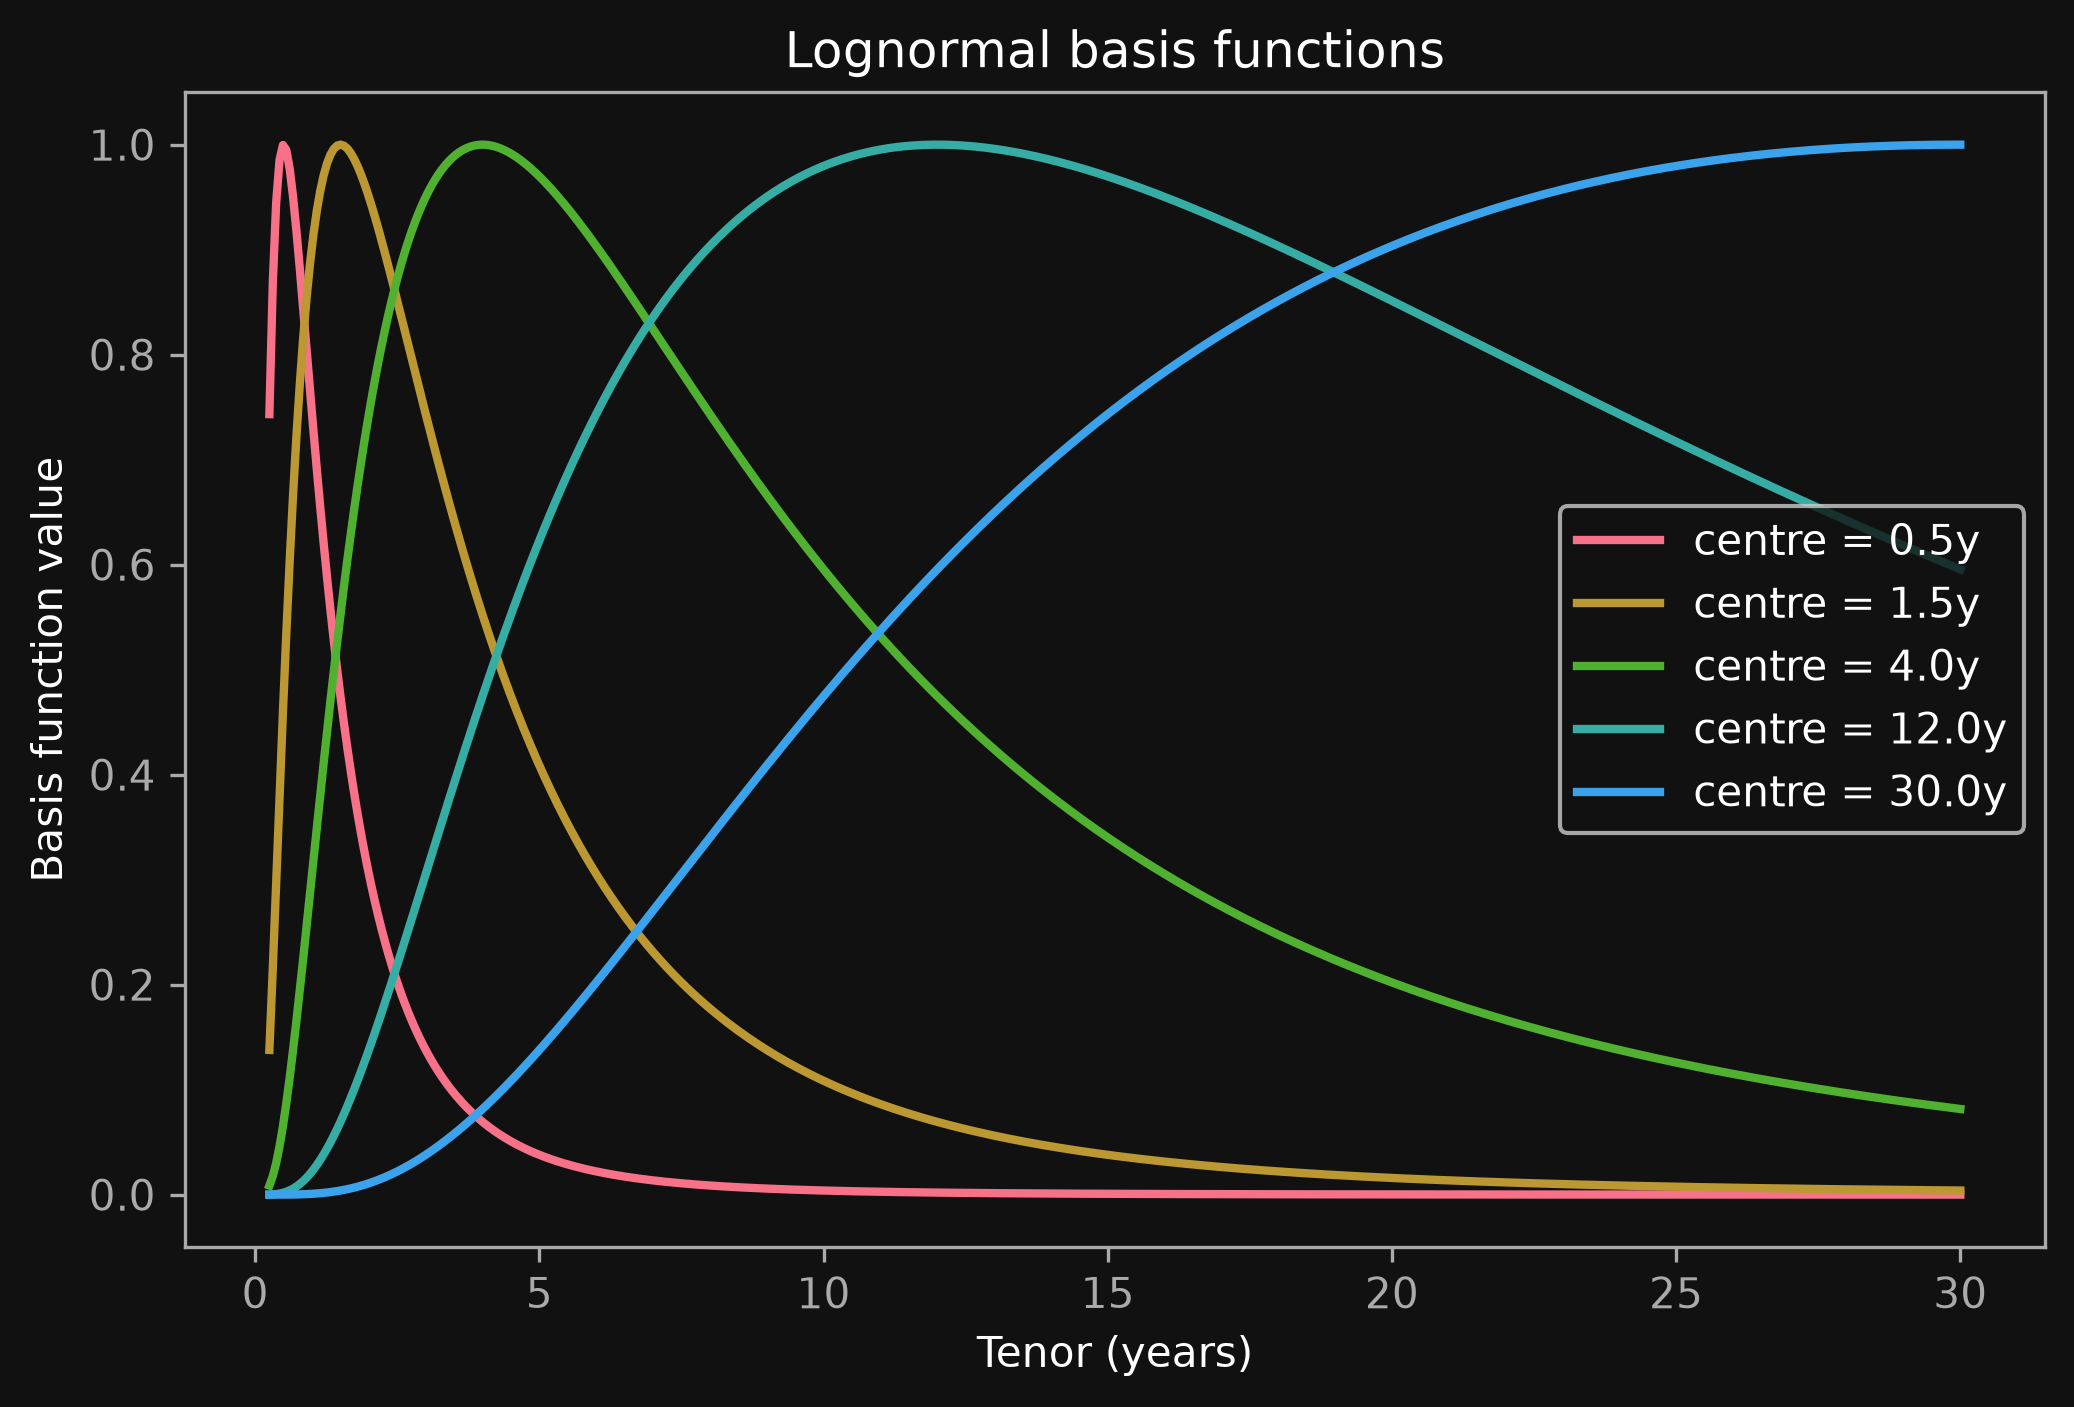
\includegraphics[width=0.68\textwidth]{./figures/problem3_basis.png}
\end{center}

$\phi_i(\tau) \ge 0.5$ when $(\log \tau - \mu_i)^2 \le 2 s^2 \log 2$, so the half-max range is
$\tau \in \left[ e^{\mu_i - s\sqrt{2\log 2}},\ e^{\mu_i + s\sqrt{2\log 2}} \right]$, a fixed ratio of
$e^{\pm 1.06}$ around the centre. Measured on \texttt{tau\_fine}, which stops at $0.25$ and $30$:

\begin{center}
\begin{tabular}{rrrrr}
\toprule
centre & on the grid & width & exact & width \\
\midrule
0.5y  & 0.25 -- 1.44  & \textbf{1.19} & 0.17 -- 1.44  & 1.27 \\
1.5y  & 0.55 -- 4.30  & 3.76 & 0.52 -- 4.33  & 3.81 \\
4y    & 1.44 -- 11.52 & 10.08 & 1.39 -- 11.54 & 10.16 \\
12y   & 4.18 -- 30.00 & 25.82 & 4.16 -- 34.62 & 30.47 \\
30y   & 10.44 -- 30.00 & \textbf{19.56} & 10.40 -- 86.56 & 76.17 \\
\bottomrule
\end{tabular}
\end{center}

The blob at 0.5 years is about $1.2$ years wide. The blob at 30 years is at least $19.6$ years wide
on the grid, and $76$ years wide if you do not stop at the 30-year point. Either way it is the blob
at the front that is narrow, which is the point of working in $\log \tau$: the basis is fine where
the curve moves and coarse where it does not.


\subproblem{3.2: Ordinary Least Squares}
Fit the five weights with OLS on \texttt{A3} and \texttt{y3}. Store them as \texttt{w\_ols3}.
\begin{itemize}
    \item Give the five weights, and the number of them that are negative.
    \item In one sentence, why is a negative weight hard to explain when each basis function is a blob of yield?
\end{itemize}

\answer

\begin{center}
\begin{tabular}{lrrrrr}
\toprule
centre & 0.5y & 1.5y & 4y & 12y & 30y \\
\midrule
$\hat w$ & 0.03083 & $\mathbf{-0.00688}$ & 0.04134 & $\mathbf{-0.00927}$ & 0.07430 \\
\bottomrule
\end{tabular}
\end{center}

\textbf{2 of the 5 weights are negative.} The smallest is $-0.00927$.

Each basis function is a blob of yield sitting at one tenor, so a negative weight says the blob at
1.5 years and the blob at 12 years \textit{remove} yield. Nothing in the market does that, and once
a weight can go negative it stops answering the question the basis was built to answer -- how much
curve sits at each tenor.


\subproblem{3.3: Non-Negative Weights}
In class we said that we could stop the negative weights with the rule $w \ge 0$. Apply that rule:

    \begin{lstlisting}[language=Python]
from scipy.optimize import minimize, nnls

res = minimize(lambda w: np.sum((A3 @ w - y3) ** 2), np.maximum(w_ols3, 0.0),
               method="L-BFGS-B", bounds=[(0.0, None)] * A3.shape[1],
               options={"maxiter": 100000, "ftol": 1e-18, "gtol": 1e-14})\end{lstlisting}

\begin{itemize}
    \item Give the five new weights.
    \item Give the RMSE against \texttt{true\_curve(tau\_fine)}.
    \item Plot your two fitted yield curves against the data, which do you think looks better?
\end{itemize}

\answer

\begin{center}
\begin{tabular}{lrrrrr}
\toprule
centre & 0.5y & 1.5y & 4y & 12y & 30y \\
\midrule
$\hat w$ & 0.02765 & \textbf{0.00000} & 0.03268 & \textbf{0.00000} & 0.06763 \\
\bottomrule
\end{tabular}
\end{center}

The two weights that were negative are now exactly zero. The rule does not shrink them, it removes
those two basis functions from the model. \texttt{scipy.optimize.nnls} returns the same answer to
$4.05 \times 10^{-9}$, so the bounded solver found the true optimum.

RMSE against \texttt{true\_curve(tau\_fine)} is $\mathbf{19.87}$ bp, against $16.70$ bp for
unconstrained OLS, and the SSE against \texttt{y3} is $1.373$ times the OLS value.

\begin{center}
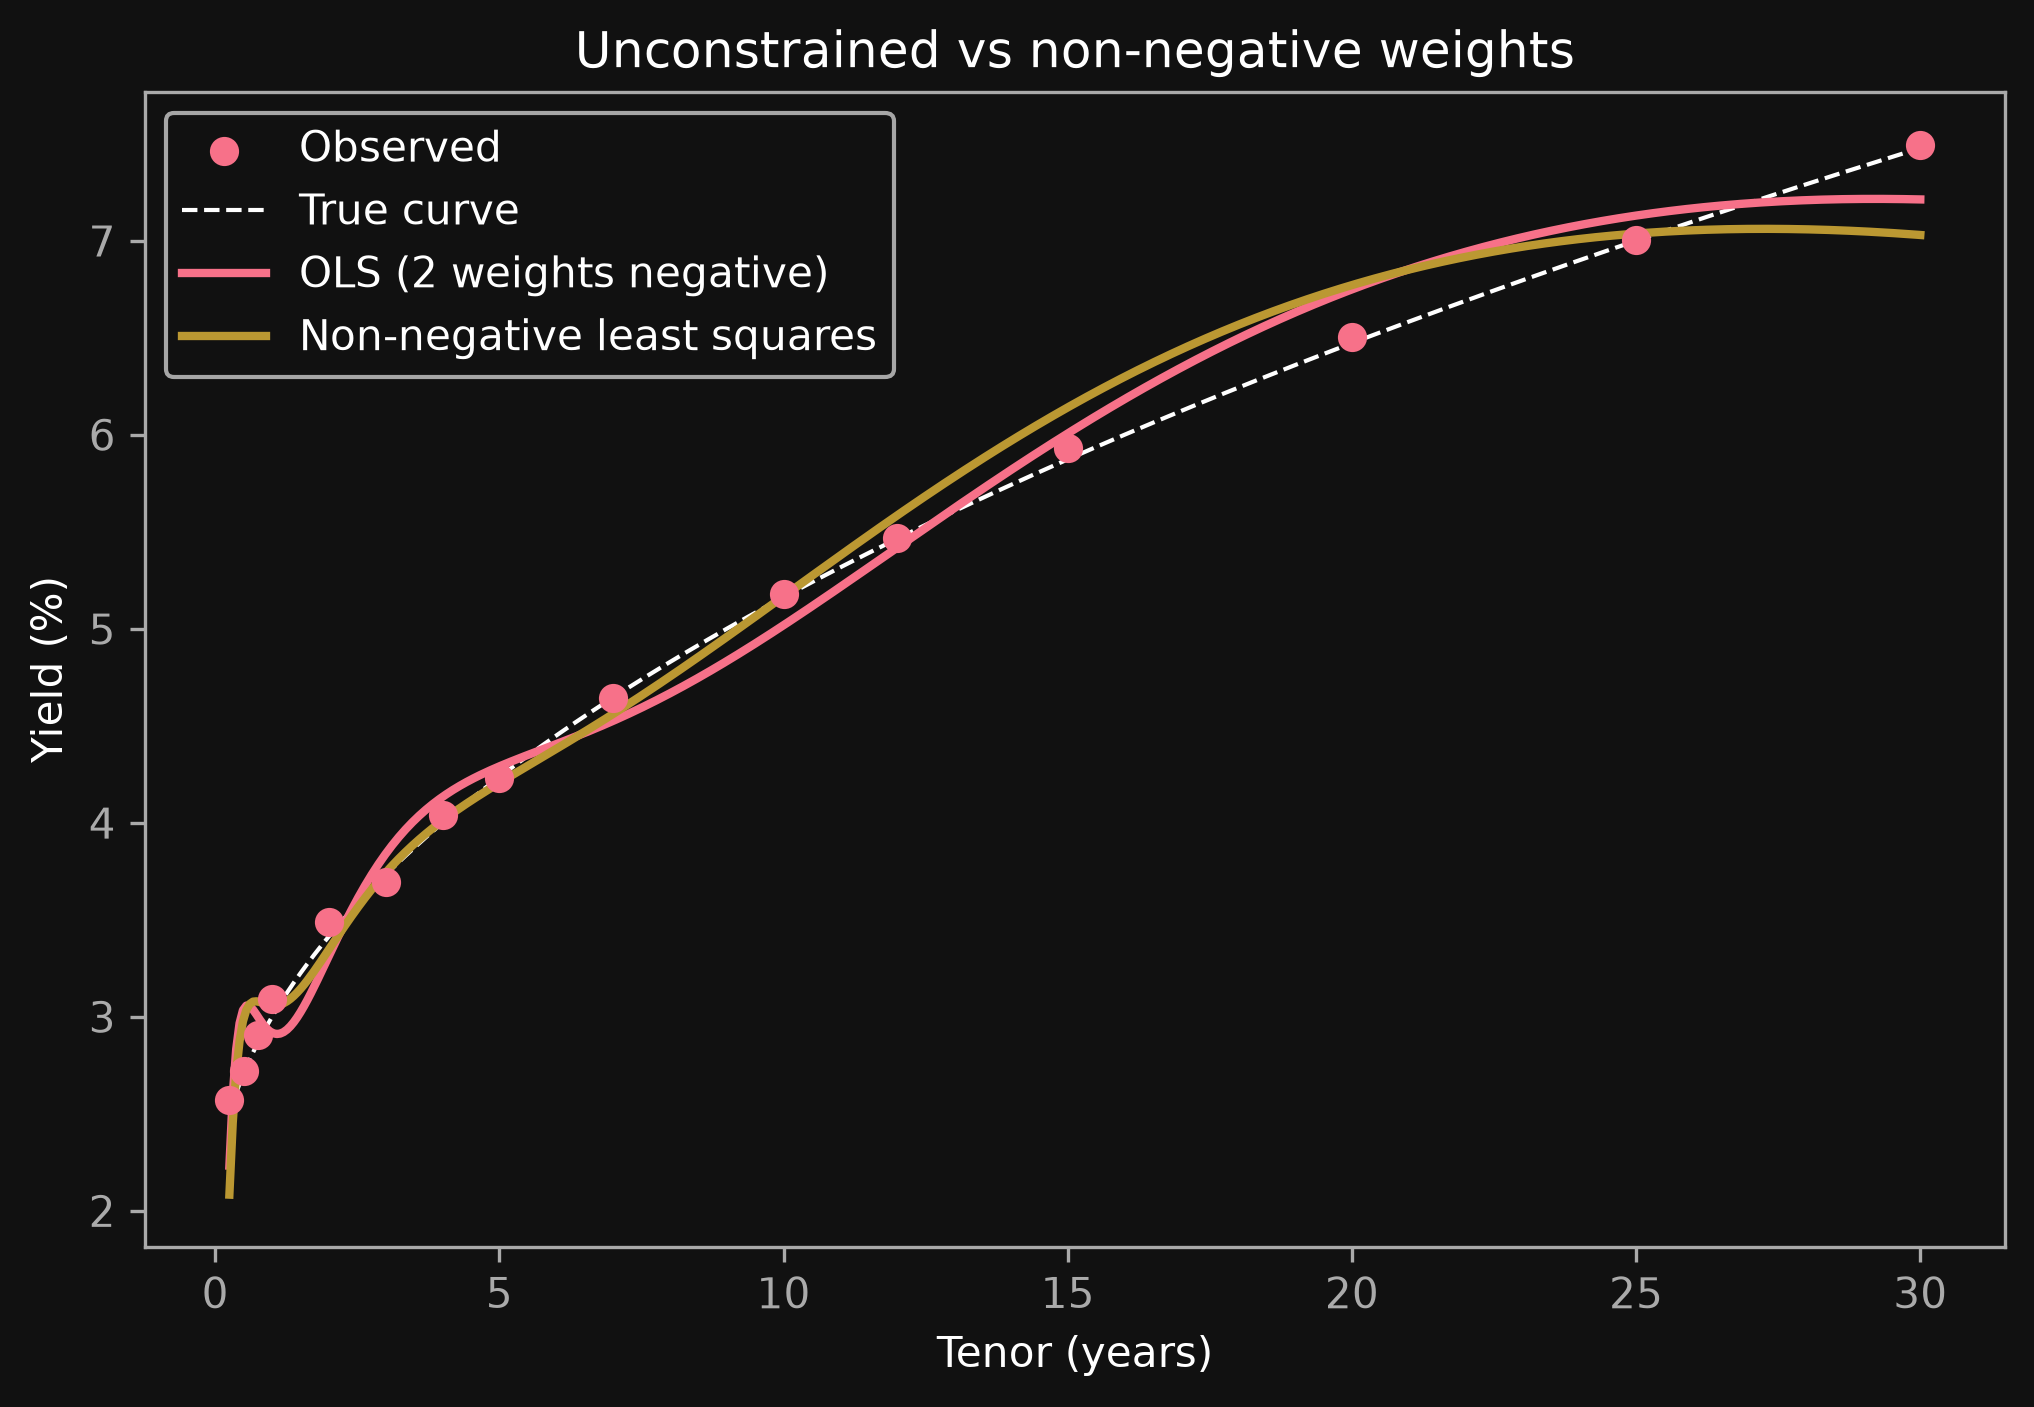
\includegraphics[width=0.68\textwidth]{./figures/problem3_fits.png}
\end{center}

\begin{center}
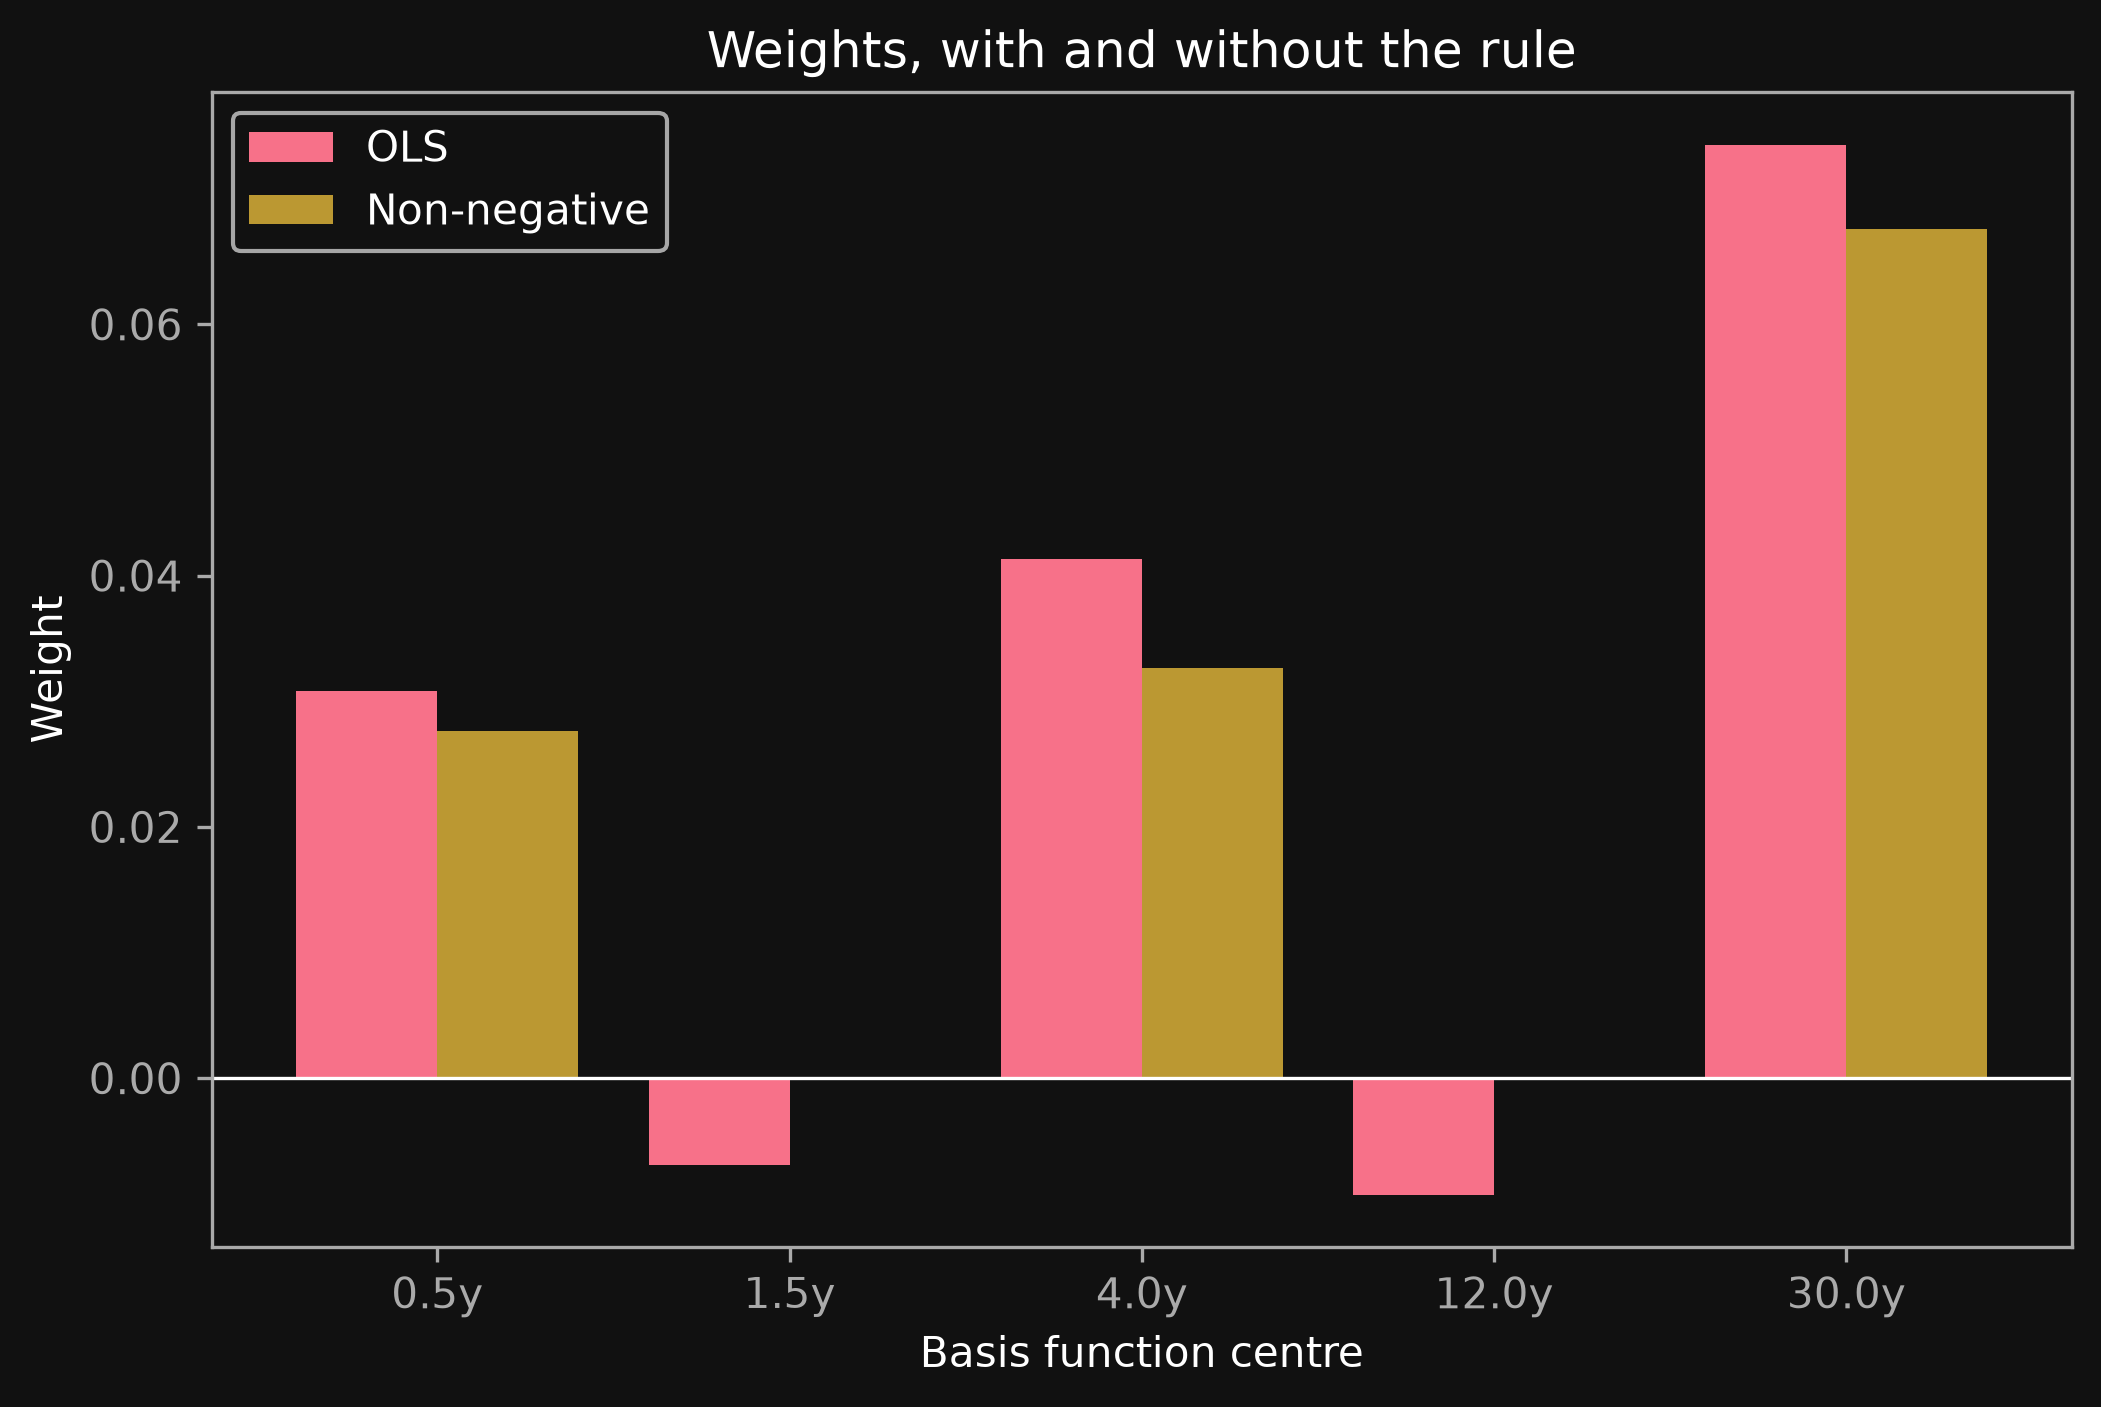
\includegraphics[width=0.68\textwidth]{./figures/problem3_weights.png}
\end{center}

The constraint costs accuracy on both measures. On the SSE against \texttt{y3} it has to: OLS
already minimizes that, and the constrained fit is a restriction of the same problem. On the RMSE
against the true curve it does not have to -- a constraint that happens to point at the truth can
help -- but here it does not. The two curves are hard to tell apart by eye, and both track the
data. The non-negative one is the better answer anyway, because the
five weights it returns can be read as an allocation across tenors and the OLS weights cannot. If
all you want is a curve, take OLS; if you want the weights to mean something, pay the $3$ bp.


\pagebreak

\problem{4: Switching Up Losses}

Sometimes, data might have bad values.

    \begin{lstlisting}[language=Python]
x4 = np.linspace(0, 1, 120)
clean_curve = np.sin(2 * np.pi * x4)

rng = np.random.RandomState(5)
y4 = clean_curve + rng.normal(0, 0.05, 120)
bad_idx = rng.choice(120, 8, replace=False)
y4[bad_idx] += rng.choice([-1, 1], 8) * 1.5     # 8 bad values

B4 = basis(x4, knots(8))          # 10 parameters
w_ols = fit_ols(B4, y4)           # the start point for both fits below\end{lstlisting}

Use these settings for every fit in this problem. Start each fit from the OLS answer.

    \begin{lstlisting}[language=Python]
from scipy.optimize import minimize

OPT = {"maxiter": 50000, "maxfun": 200000, "ftol": 1e-15, "gtol": 1e-12}
# minimize(loss, w_ols, method="L-BFGS-B", options=OPT)\end{lstlisting}

\subproblem{4.1: Least Squares}
Plot the data, the OLS curve, and \texttt{clean\_curve} on one set of axes. Show the 8 bad values in a different color.

\answer

The 8 bad values are at index $21, 41, 48, 63, 65, 66, 95, 98$.

\begin{center}
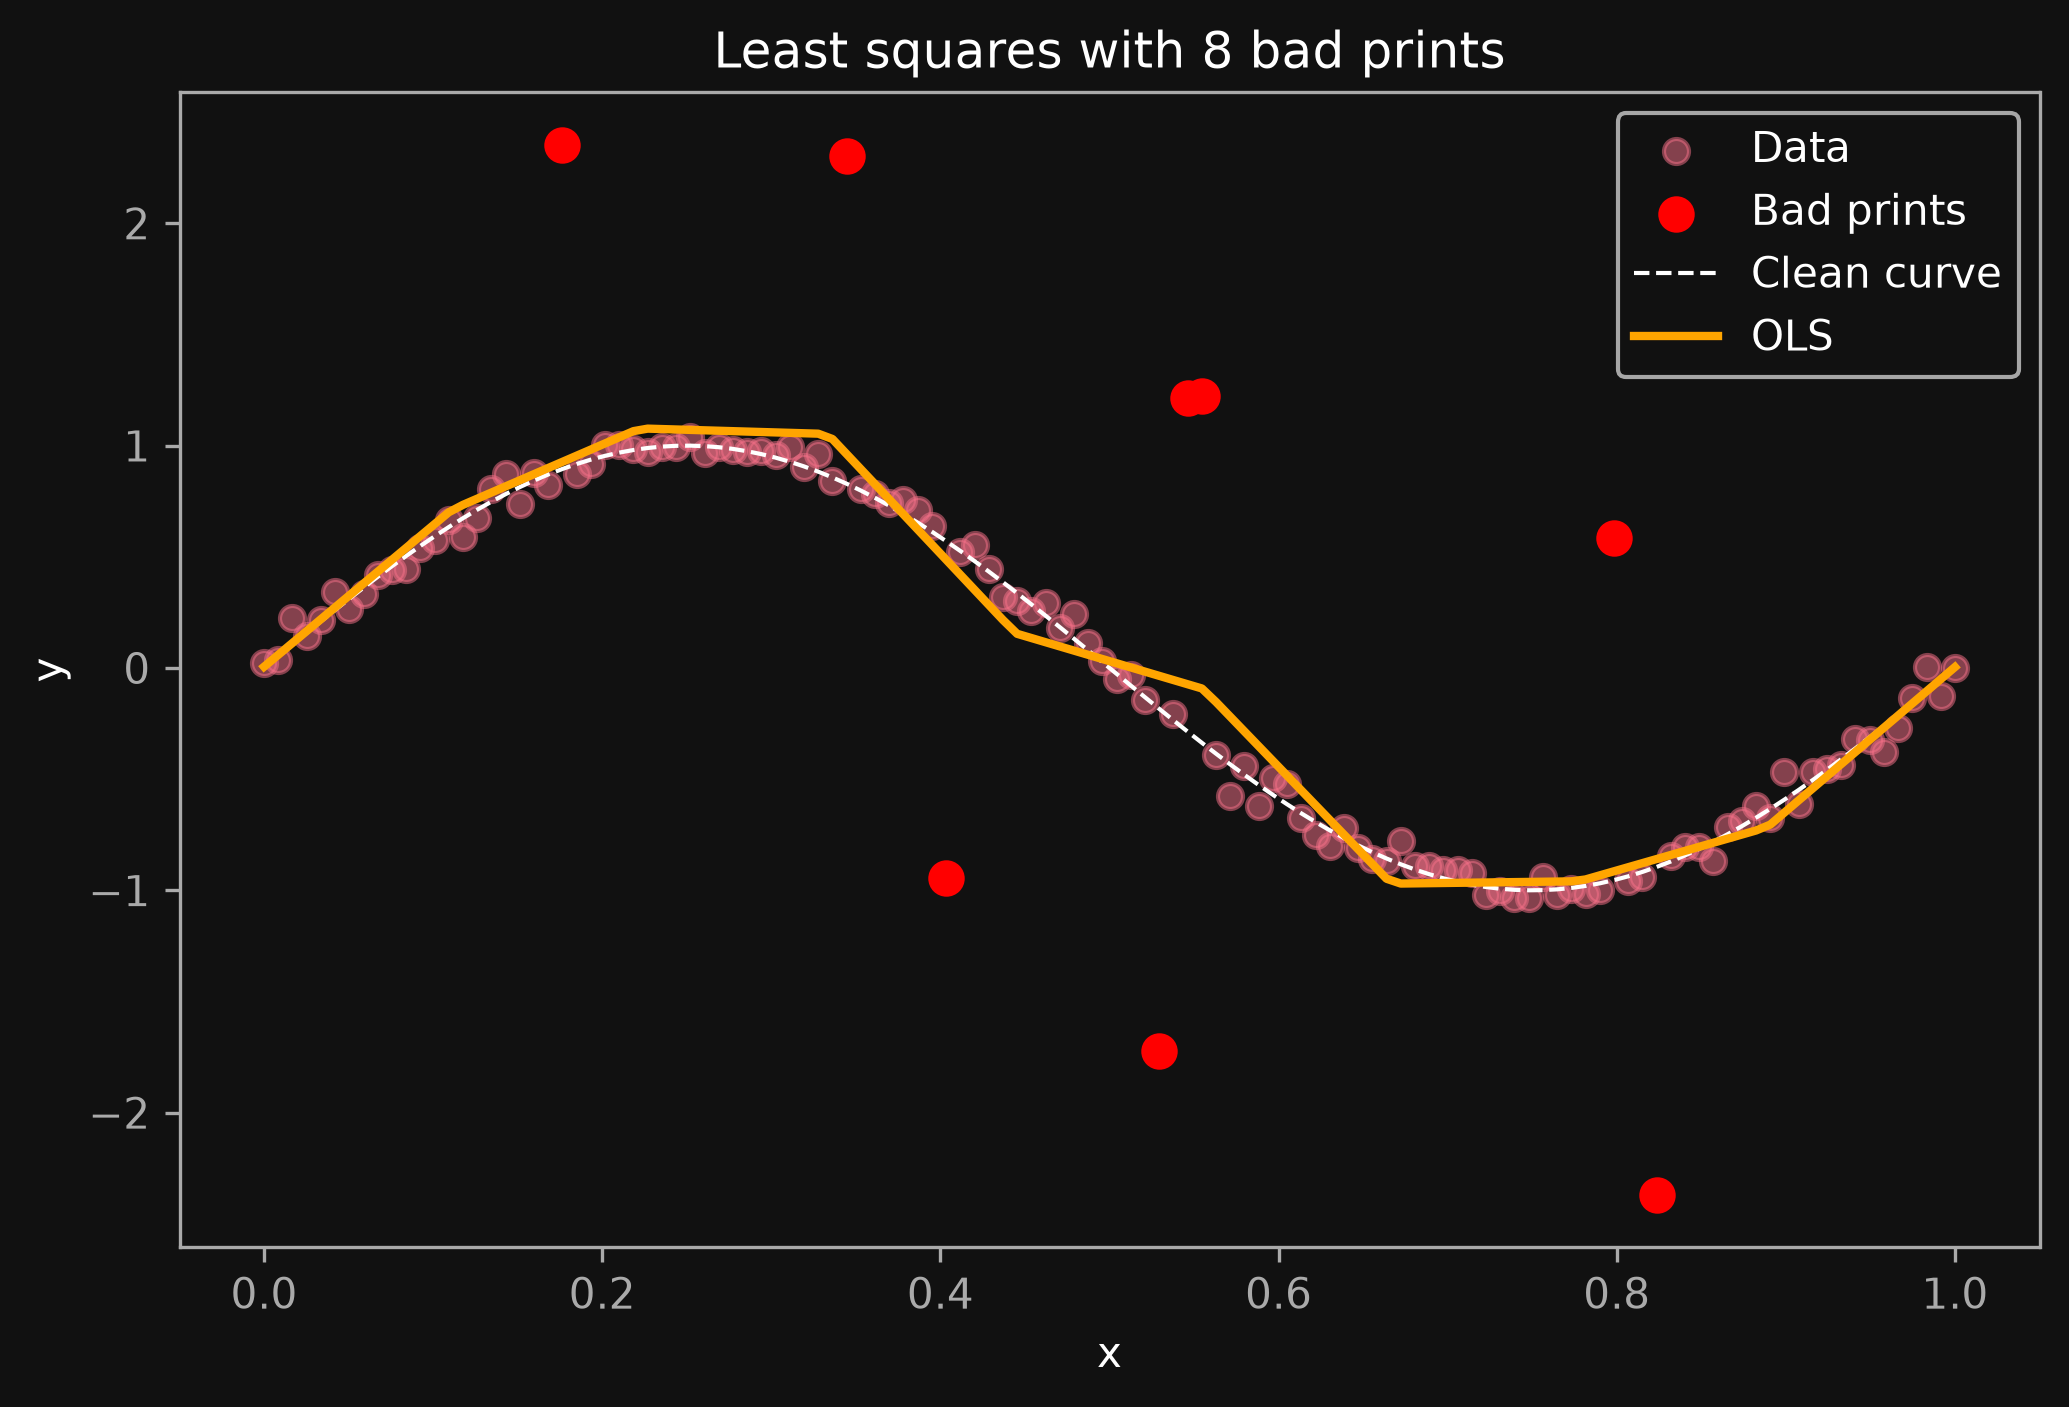
\includegraphics[width=0.68\textwidth]{./figures/problem4_ols.png}
\end{center}

The curve moves toward every bad value.


\subproblem{4.2: Two Other Losses}
Write these two losses yourself, then run them through \texttt{scipy.optimize.minimize}:
\begin{itemize}
    \item the Huber loss with $\delta = 0.1$:
    $$
    \rho_\delta(r) = \begin{cases}
        \tfrac{1}{2} r^2 & |r| \le \delta \\[2pt]
        \delta \left( |r| - \tfrac{1}{2}\delta \right) & |r| > \delta
    \end{cases}
    $$
    \item the (almost) absolute loss. Use the smooth version below (so that it's differentiable at $r=0$).
    $$
    \rho(r) = \sqrt{r^2 + \varepsilon^2}, \qquad \varepsilon = 10^{-3}
    $$
\end{itemize}
Plot these two curves and the OLS curve from 4.1 together with \texttt{clean\_curve}.

\answer

\begin{lstlisting}[language=Python]
def huber_loss(r, delta):
    a = np.abs(r)
    return np.where(a <= delta, 0.5 * r**2, delta * (a - 0.5 * delta))

w_huber = minimize(lambda w: np.sum(huber_loss(B4 @ w - y4, 0.1)), w_ols,
                   method="L-BFGS-B", options=OPT).x

# |r| has a sharp corner at 0 that a solver cannot follow, so smooth it slightly
w_abs = minimize(lambda w: np.sum(np.sqrt((B4 @ w - y4) ** 2 + EPS**2)), w_ols,
                 method="L-BFGS-B", options=OPT).x
\end{lstlisting}

\begin{center}
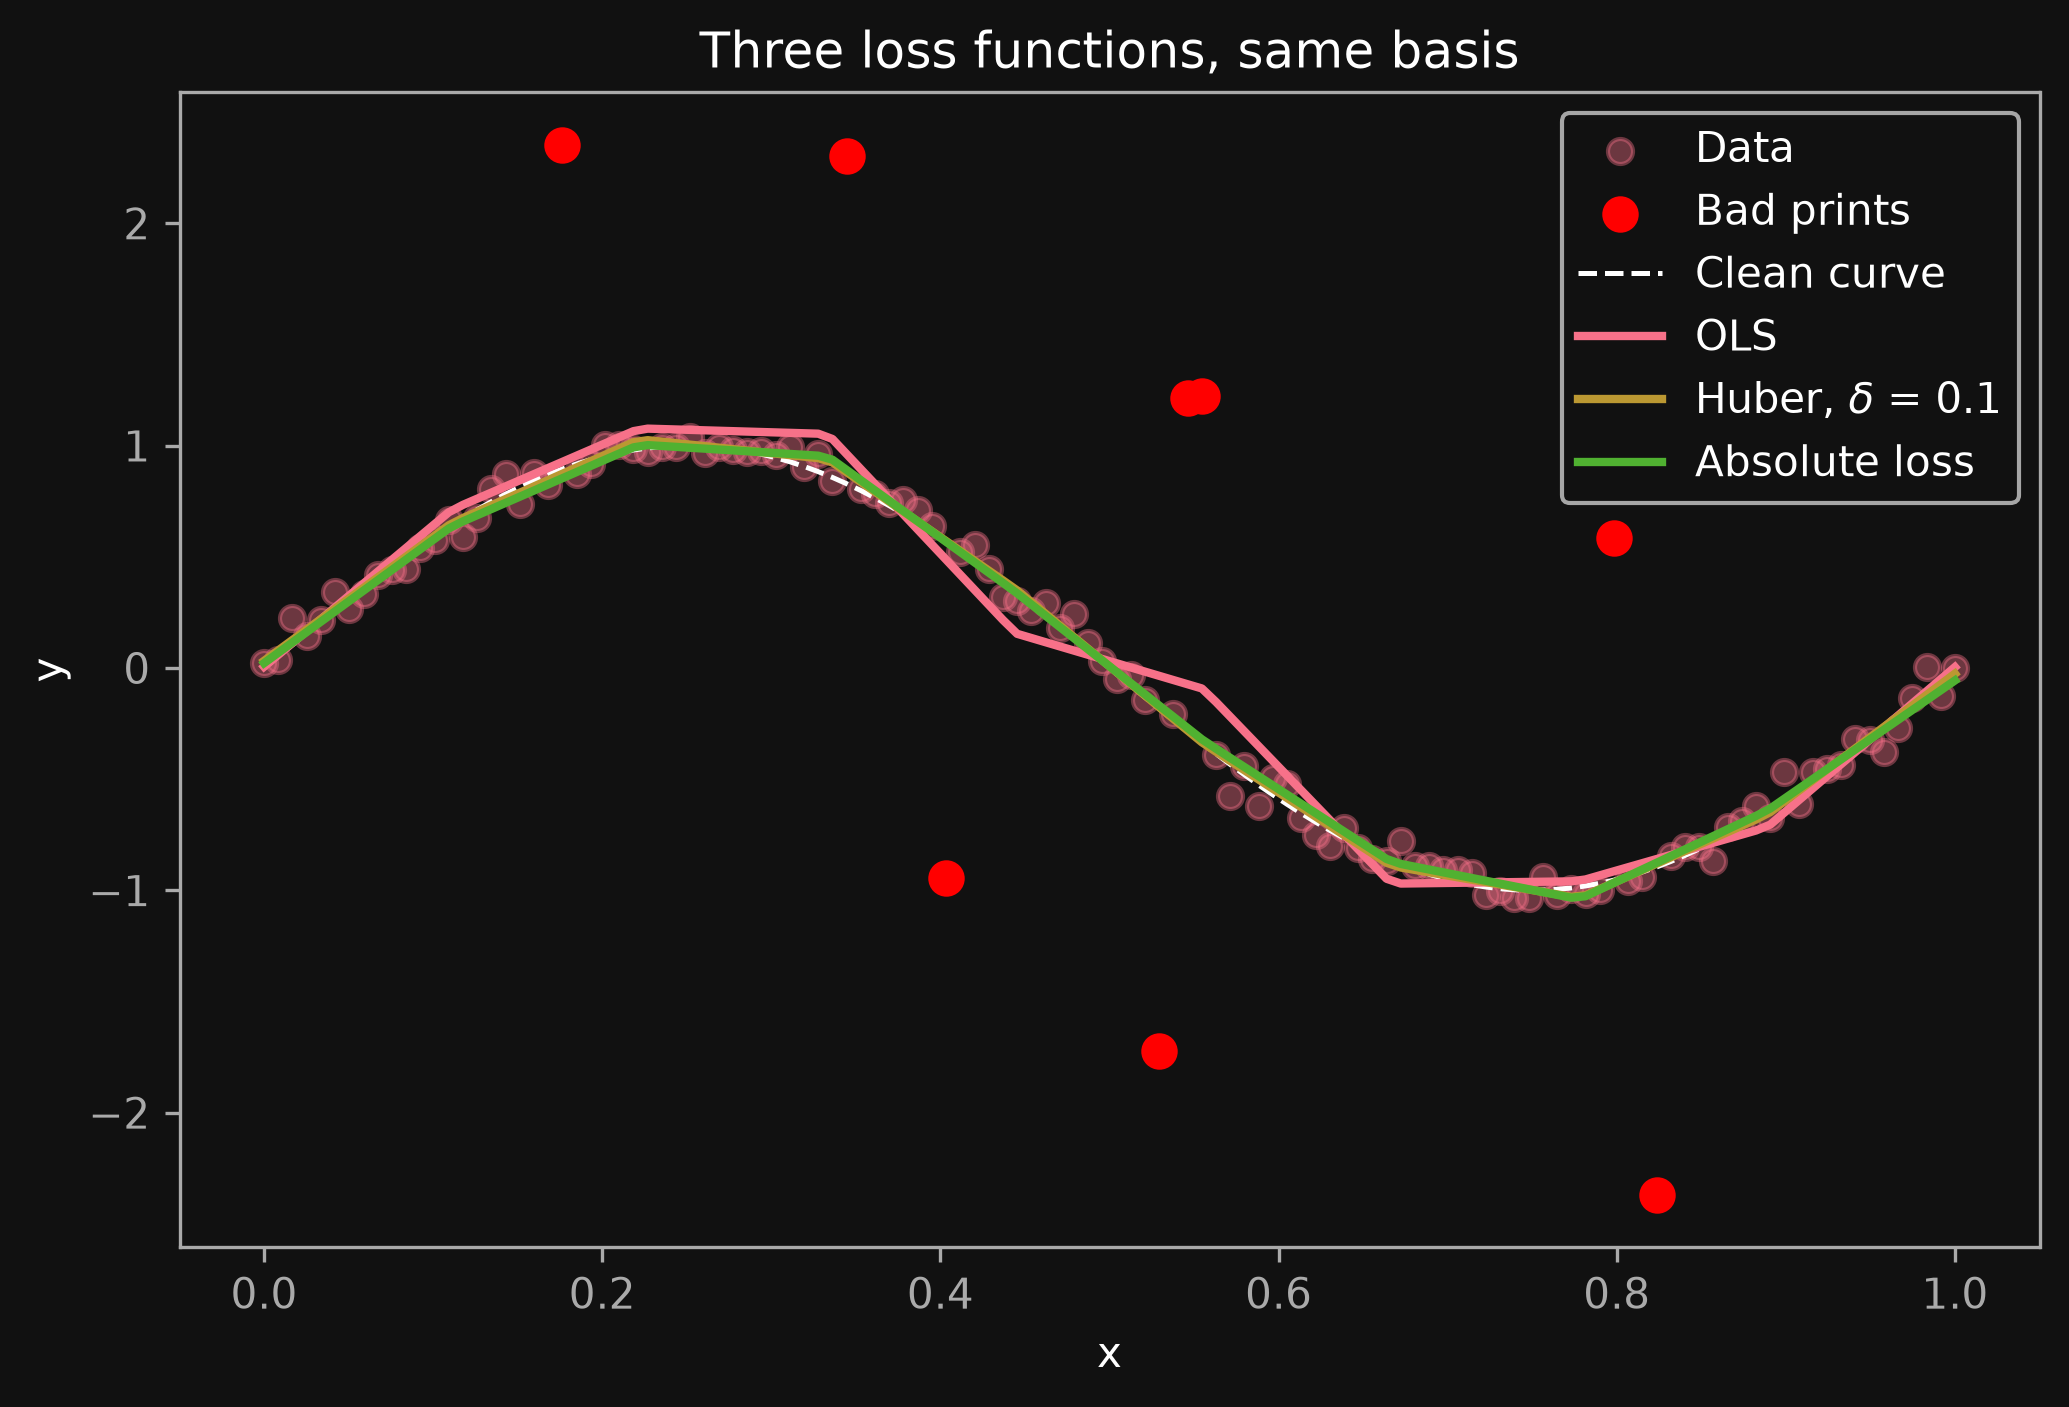
\includegraphics[width=0.68\textwidth]{./figures/problem4_losses.png}
\end{center}

The smoothing matters. With the sharp corner left in place, a gradient-based solver stops early and
returns a worse answer than the true minimum of $\sum |r|$.


\subproblem{4.3: Which Loss Wins}
\begin{itemize}
    \item Give the RMSE of the three fits against \texttt{clean\_curve}.
    \item Which one is lowest, and why?
    \item Now give the RMSE of the three fits against \texttt{y4} as well. Which is better, and why do you think that is?
\end{itemize}

\answer

\begin{center}
\begin{tabular}{lrr}
\toprule
loss & RMSE vs clean curve & RMSE vs \texttt{y4} \\
\midrule
OLS      & 0.0860 & \textbf{0.3844} \\
Huber ($\delta = 0.1$) & \textbf{0.0190} & 0.3926 \\
absolute & 0.0257 & 0.3927 \\
\bottomrule
\end{tabular}
\end{center}

\textbf{Huber wins on the clean curve}, at $0.0190$ against $0.0257$ for the absolute loss and
$0.0860$ for OLS.

Squared error grows with $r^2$, so a distant point dominates the objective and the curve must move
toward it. Compare the share of the objective that a residual of $1.5$ takes against one of $0.1$:
OLS gives it $225\times$ the weight, Huber $29\times$, the absolute loss only $15\times$.

Huber wins because it does both jobs at once. It is quadratic near zero, so it uses the 112 good
points as efficiently as OLS does, and linear far out, so the 8 bad values get a bounded vote. The
absolute loss is linear everywhere: it handles the bad values but throws away the same information
on the good points, so it lands between OLS and Huber.

\textbf{OLS wins on \texttt{y4} and loses on the clean curve.} That ordering is guaranteed, not
luck: OLS minimizes the squared error against \texttt{y4} by construction, so nothing can beat it
there -- and \texttt{y4} is the series that holds the 8 bad values. Fitting the data you were given
and fitting the process that generated it are not the same objective.


\subproblem{4.4: The Effect of $\delta$}
Fit the Huber loss again for $\delta \in \{0.01,\, 0.05,\, 0.1,\, 0.5,\, 1.0,\, 5.0\}$.
\begin{itemize}
    \item Give the RMSE against \texttt{clean\_curve} for each $\delta$.
    \item What is Huber loss like for very small $\delta$? And what is it like for really big $\delta$?
\end{itemize}

\answer

\begin{center}
\begin{tabular}{rrr}
\toprule
$\delta$ & RMSE vs clean curve & largest $|r|$ \\
\midrule
0.01 & 0.0228 & 1.5536 \\
0.05 & 0.0201 & 1.5525 \\
0.10 & \textbf{0.0190} & 1.5571 \\
0.50 & 0.0365 & 1.6026 \\
1.00 & 0.0710 & 1.6806 \\
5.00 & 0.0860 & 1.6895 \\
\bottomrule
\end{tabular}
\end{center}

As $\delta \to 0$ Huber becomes the \textbf{absolute loss}; as $\delta \to \infty$ it becomes
\textbf{OLS}.

Both ends show up in the table. At $\delta = 5.0$ the RMSE is $0.0860$, which is OLS exactly: no fit
here leaves a residual larger than $1.6895$, well below $5$, so no point ever reaches the linear part
and Huber is minimizing $\tfrac{1}{2} r^2$ everywhere. At $\delta = 0.01$ the RMSE is $0.0228$,
close to the $0.0257$ of the absolute loss.

The table has an interior minimum, at $\delta = 0.1$. Too large and Huber behaves like OLS and
chases the bad values; too small and it behaves like the absolute loss and gives up efficiency on
the good points.


\end{document}
